\section{第一章
融媒时代新型主流媒体的界定与内涵}\label{ux7b2cux4e00ux7ae0-ux878dux5a92ux65f6ux4ee3ux65b0ux578bux4e3bux6d41ux5a92ux4f53ux7684ux754cux5b9aux4e0eux5185ux6db5}

2014年8月18日，习近平总书记在主持召开中央全面深化改革领导小组第四次会议并发表重要讲话时要求，推动传统媒体和新兴媒体在内容、渠道、平台、经营、管理等方面的深度融合，着力打造一批形态多样、手段先进、具有竞争力的新型主流媒体，建成几家拥有强大实力和传播力、公信力、影响力的新型媒体集团，形成立体多样、融合发展的现代传播体系。\footnote{新华社.
  (2014). 习近平主持召开中央全面深化改革领导小组第四次会议. 中国政府网,
  https://www.gov.cn/xinwen/2014-08/18/content\_2736451.html,
  2025年5月11日访问.}自此之后，推动建设具有``融媒性质''的新型主流媒体成为国家政治议程中的重要一环。

随后中国传统主流媒体便积极响应号召，不断适应社会信息化持续推动的新情况，运用新技术与新应用，创新媒体传播方式，打造新型传播平台，通过媒介融合的方式建设新型主流媒体。发展至今，我国的媒体融合建设已由初步探索进入纵深发展阶段。而正如高钢早在2007年所指出的，媒体融合并非定态目标，而是一个动态过程，其总随着现代信息技术推进对信息传播的技术手段、功能结构和形态模式的改变而改变，\footnote{高钢.
  (2007). 媒体融合：追求信息传播理想境界的过程. 国际新闻界，3, 54-59,
  pp.54-55.}融媒技术特征在传统主流媒体向新型主流媒体转型的过程贯穿始终。如要对中国环境传播主流话语在近年的历时性变化进行深入阐发，首先需要对新型主流媒体及其融媒技术特性进行解读说明。

主流媒体这一概念的最早提出源于美国语言学家乔姆斯基（Noam
Chomsky），在他的定义下，具有报道严肃、解剖深入、信誉卓著、社会地位高等特征，同时具备为社会进行议程设置的功能的媒体即为传统时代的主流媒体。\footnote{Chomsky,
  N. (1997). What makes mainstream media mainstream. Z magazine, 10(10),
  17-23.}而相比于西方视野下的定义，我国主流媒体更多还要考虑其对于主流意识形态的代表作用，要求其具有强大影响力与舆论引导力，在传播中成为承载正能量的载体。\footnote{匡文波，马茜茜.
  (2019).
  媒体融合环境下的对外传播策略------解读习总书记``1·25''关于媒体融合的讲话精神.
  对外传播, 5, 8-9+1, p.8.}美国学者罗杰·菲德勒（Roger
Fidler）在《媒介形态变化------认识新媒介》（Mediamorphosis：Understanding
New
Media）一书中指出，新的传播媒介形式往往也会继承与发扬旧有媒介形式的主要特点，\footnote{罗杰·菲德勒.
  (2000). 《媒介形态变化------认识新媒介》.明安香译. 华夏出版社,pp.24.}新型主流媒体在发展过程中仍承袭了传统主流媒体在大众传播时代所具备的政治、意识形态属性，以及较高的媒体生态地位等突出特征。同时，伴随现代信息技术的发展，尤其是数字化、网络化和移动互联网的普及，传统主流媒体的传播模式面临前所未有的挑战，因而催发其在媒介形式上产生变革，在原有的基础上融入新兴媒体的内涵，向新型主流媒体进行转型。

新型主流媒体脱胎于传统主流媒体，但并非只是传统主流媒体与新兴技术的简单结合，而是更多利用技术在内容创造和叙事表征方式实现深层次的突破。新型主流媒体构建的传播模式全面而立体，能够将信息多元呈现，其兼顾新媒体的技术优势和主流媒体的功能与属性，
是既拥有强大实力、传播力、公信力和影响力，又具备形态多样、手段先进、竞争力等特征的新时代下的主流媒体。

新型主流媒体的融合媒介发展，指的是新型主流媒体为适应信息传播技术发展，在媒体形式、传播方式、平台和渠道的深度融合，其在融会贯通各项传播优势的同时，也派生出诸多的融媒特性。而相较于传统主流媒体，新型主流媒体在融合媒体发展中展现出的技术特性格外突出。在我国新型主流媒体的环境话语传播中，其融媒技术特性对于传统环境报道的革新显著可见，其主要集中于以下表现：多平台融合传播、实时反馈、叙事表征方式融合。

首先，在传统大众传播时代，环境信息传播往往依赖于电视、广播、报纸等单一媒介平台。而随着数字移动通讯技术和互联网信息平台的繁盛，环境信息的承载方式越发多元。新型主流媒体在进行技术改造的同时，并未舍弃固有的信息传播渠道，而是在保持传统媒体运行机制的基础上添加各种新媒体形态及内容分发渠道，以求在变化中更合理地重新配置媒体资源。\footnote{蔡雯.
  (2020).
  媒体融合进程中的``连接''与``开放''------兼论新型主流媒体建设的难点突破.
  国际新闻界, 42(10), 6-17, pp.8-9.}这便呈现出新型主流媒体多平台传播的融媒发展特征------以《人民日报》为例，其基于社交媒体平台与短视频平台进行内容传播，也继续在报纸版面上进行内容生产，并通过电视和广播进行大众宣传。

新型主流媒体在运营模式和组织结构上进行了调整与创新，通过多平台传播同一类型信息，使新闻信息的传播能做到更迅速、更全面、更立体------将环境信息传播途径进行了综合拓展，进而使得其对受众的覆盖面显著提升。

其次，互联网传播时代，时空界限被打破，信息一经上网，在理论上便是无远弗届的全球传播。\footnote{喻国明.
  (2019).
  今天的媒介融合应当怎么做------从互联网时代的常识到新传播格局的大势.
  教育传媒研究, 4, 7-9, p.7.}在当代信息技术发展下，新闻报道的延时性大大降低，信息的即时性相应提高。尤其是在社交平台和短视频平台上，突发环境新闻甚至可以在几分钟内得到全球范围的传播。这种即时性提高了新闻的时效性和覆盖面，使得新闻能够快速响应社会事件、回应公众需求。

而与此相伴随的是实时反馈机制。当主流媒体在互联网平台发布环境新闻信息，受众的评论、点赞和分享等互动反馈可以直接影响新闻的传播效果，给予发布者可以被量化观测的反馈------通过分析受众的反馈，主流媒体能够实时调整报道内容和传播策略：选择或是进一步扩展报道内容，或是通过后续报道跟进事件进展，或是从受众视角对相关新闻进行新的补足。

最后，媒介呈现技术的变化显著地引起了环境新闻叙事表征方式的融合。在传统的新闻报道中，环境信息的呈现通常依赖于文字和图片，而现代融媒技术通过引入视频、音频、动画等多重媒介元素，同以往的叙事表征方式进行结合，使得信息传播呈现出更多维度------在讨论气候变化的议题时，单一的文字新闻可能无法全面展现这一复杂问题，而通过图表和视频，使得气候变化的数据趋势可以被清晰地数据化和可视化。视频将直接呈现生态破坏和保护的结果，实时的数据图表将具体化空气污染的程度，动画则将清晰呈现城市生态系统的变迁过程。新型主流媒体利用融媒技术丰富了环境相关叙事的表征方式，但同时，也意味着环境叙事传达与感知日益趋向于复杂。如何有效地组织媒介元素进行环境叙事表达，使受众能清晰认知到传播意图、受到环境话语宣传的影响，成为新型主流媒体进行环境传播实践需要思考的问题。

\section{第二章
新中国75周年主流媒体报道环境的话语特征与演变------以《人民日报》为例}\label{ux7b2cux4e8cux7ae0-ux65b0ux4e2dux56fd75ux5468ux5e74ux4e3bux6d41ux5a92ux4f53ux62a5ux9053ux73afux5883ux7684ux8bddux8bedux7279ux5f81ux4e0eux6f14ux53d8ux4ee5ux4ebaux6c11ux65e5ux62a5ux4e3aux4f8b}

环境保护作为关乎国民民生健康，经济发展和文明永续的关键命题，在当代公共议题的讨论中被置于重要位置，并在政治顶层设计和新闻报道中得以体现。近年来，国家持续推进生态文明建设。据环境部2024年发布的环境公报，全国环境各类环境质量发展稳中向好，生态环境治理取得新成效，各类环境风险得到基本管控，生态质量指数达59.6，生态质量综合评价为``二类''，自然生态状况总体稳定。\footnote{中华人民共和国生态环境部.
  (2024). 《2023中国生态环境状况公报》, 1-82,pp.1-2.}在对中国现代化历史进行考量后，我们不难发现，环境保护话语的重要程度伴随社会变迁，步步上升，现已成为我国关乎全民健康福祉、经济发展与回应人类命运共同体的重要战略议题。

环境话语是环境现象和观念集合的语言表征，为人们理解环境，与环境沟通和对话提供了思维工具与概念化手段，对建构、维持及改变环境现实具有重要意义，\footnote{郑红莲,王馥芳.
  (2018). 环境话语研究进展与成果综述. 北京科技大学学报(社会科学版),
  34(04), 9-16, p.9.}其并非总一成不变，而是伴随社会历史变迁的发展而变化。从新中国成立初期``向自然宣战''的征服式话语到当代``绿水青山就是金山银山''，强调经济发展同环境协调发展话语，中国环境保护的认知历经75周年漫长过程。在这个过程中，主流媒体像``明镜''一样折射出新中国成立以来中国社会对环境利用和保护管理上的观念与实践转向，又仿佛``明灯''一般\footnote{高金萍.
  (2017).
  《``明镜''与``明灯'':中国主流媒体话语与社会变迁研究》(2003-2012).
  中国人民大学出版社, pp.87-95.}通过新闻框架的建构、议程设置、象征符号编码等方法指引社会环境实践，建构中国环境议题，最终形成具有中国特色的环境话语体系。

《人民日报》自1948年创刊以来，见证并记录了新中国从成立到改革开放、再到现代化建设的历史进程。在社会影响力层面，其作为中共中央机关报，直接反映党和政府的政策导向，能够引导公众认知，建构社会舆论，对中国社会主流价值观和意识形态构建具有强大的支撑作用。在中国媒体生态层面，其报道内容和叙事框架深刻影响国内其他新闻媒体的内容生产和议程设置，能够代表或左右舆论，在主流媒体阵地中具有代表性。\footnote{周胜林.
  (2001). 论主流媒介. 新闻界,2001(06), 11-12, p.11.}于样本内容层面考虑，《人民日报》数据库存留有1948年创刊迄今完整的纸面新闻报道资料，将其作为分析对象，能够完整地呈现新中国成立以来主流媒体有关于环境话语变迁的全过程。

本研究将采用批评话语分析的方法，对《人民日报》75周年环境报道进行文本分析和话语实践分析，考察中国环境治理进程中新闻话语扮演的角色。在具体操作层面上，采取话语分析和内容分析相结合的方式，对媒介话语进行定量研究，从而推导出社会历史的变迁和趋势\footnote{甘莅豪.
  (2011). 媒介话语分析的认知途径:中美报道南海问题的隐喻建构.国际新闻界,
  33(08),83-90, p.83.}，说明主流媒体生产的新闻话语是如何反映并建构中国环境话语。

\subsection{第一节
环境话语与媒体报道研究}\label{ux7b2cux4e00ux8282-ux73afux5883ux8bddux8bedux4e0eux5a92ux4f53ux62a5ux9053ux7814ux7a76}

20世纪60年代，随着环境问题在全球社会发展问题中逐渐显著，以环境问题为主要关注对象的新闻报道和视觉图像开始显要地出现在媒体之中，\footnote{Cox,R.
  (2006). Environmental Communication and Public Sphere. London: Sage,
  pp.115-117.}环境议题借助媒介表达开始逐渐深入公共领域。在这一背景之下，关于环境问题的讨论和环境保护的各类实践活动开始兴起，投射到传播学科上，催生了环境传播这一分支领域的发展。自上世纪60年代环境传播起步到今天，``环境传播''的概念历经了一系列学科沉淀逐渐形成。虽然在``环境传播是什么''的概念认知上，环境传播学者们有些许分歧，但对于环境传播在回应环境议题和再建构社会环境符号和意义上的作用能够大体达成一致。\footnote{刘涛.
  (2016).
  ``传播环境''还是``环境传播''?------环境传播的学术起源与意义框架.
  新闻与传播研究, 23(07), 110-125, pp.110-114.}在``环境传播研究什么''上，苏珊·塞内卡（Susan
L.
Senecah）等学者，将环境传播的研究对象重点设置为``环境与传播之间一切可能的知识话语''，\footnote{Senecah,S.L.
  (2004). The Environmental Communication Yearbook (vol.1), London:
  Routledge, p.vii.}注重以社会环境议题中被各类主体生产的知识话语，例如把媒介生产出的新闻文本作为研究对象。罗伯特·考克斯（Robert
Cox）在其专著《环境传播与公共领域》（Environmental Communication and
Public
Sphere）中，鉴于新闻工作者和主流媒体在对于大众环境信息接受的感知层面上的重要影响作用，也将媒介和环境新闻看作是环境传播研究领域的七分之一。\footnote{Cox,R.
  (2006). Environmental Communication and Public Sphere. London: Sage,
  pp.36-37.}

纵观我国环境传播研究发展历程，学者们也多关注以大众媒介为代表的社会传播行为及其生产文本------这与大众媒介在中国社会环境议题建构中的核心地位密不可分。在梵·迪克（Van
Dijk）看来，新闻话语并不仅仅是传递信息的载体，其必然表达和确认其制作者的社会和政治态度。\footnote{Van
  Dijk,T. (1988). News As Discourse. London: Routledge, p.75.}媒介机构，尤其是具有广泛影响力的主流媒体，通过对新闻文本内容的塑造，能够影响公众的认知模式和社会共识的形成，从而参与到社会现实的建构与权力的运作之中。换言之，媒介选择什么样的内容和形式来生产新闻，直接关系到社会环境议题的建构、公众对环境风险的感知、对环境政策的态度以及环境保护实践的动员。

因此，考察新闻媒介------特别是主流媒体的环境话语实践在中国环境传播研究中具有特殊的重要性。在中国语境下的主流媒体，特别是党报体系核心媒体，对于话语构建具有更为复杂和关键的作用，其不仅是信息发布平台，更是党和国家路线、方针、政策的重要宣传阵地，对主流价值观构建起决定性影响和主要支撑作用，\footnote{林晖.
  (2008). 中国主流媒体与主流价值观之构建. 新闻与传播研究, (02),
  41-47+94, pp.41-42.}其受到``政府主导''模式的影响，承担着环保宣导和舆论监督的重要职责。\footnote{王利涛.
  (2011). 从政府主导到公共性重建------中国环境新闻发展的困境与前景.
  中国地质大学学报(社会科学版), 11(01), 76-81, pp.78-79.}通过观察《人民日报》环境话语的变迁，可以对中国主流媒体环境报道话语特征、国家环境治理逻辑以及环境保护层面的主流意识形态发展过程得到透彻理解。

国内不少学者已经基于《人民日报》等主流媒体的环境报道进行了先行研究。如李娜对《人民日报》历史环境新闻报道进行了框架分析和话语分析，呈现了《人民日报》在环境新闻报道上惯用的框架选择和修辞策略，对新中国成立七十年间，主流媒体引导下的环境报道话语报道变迁进行了分期说明，揭露了环境报道话语由依靠``爱国''话语到构建``文明建设''文化话语的转变。\footnote{李娜.
  (2019). 从爱国到文明:建国70年主流媒体环境话语变迁与共意动员. 新闻界,
  (12), 38-49, pp.43-45.}马华芳则以垃圾议题为切入点，对《人民日报》1978年---2019年的垃圾议题报道文本分出七大报道主体，说明了社会文化层面，垃圾议题建构历经的``缺失---萌芽---发展---完善''四个历史阶段。\footnote{马华芳.
  (2020). 环境传播视域下主流媒体关于垃圾议题报道的话语变迁.
  华中师范大学, 1-49, pp.31-37.}邢雪莹同样以``垃圾''切入研究，对《人民日报》中有关垃圾分类的报道进行了议程设置研究，发现其多用政治叙事、``悲情弱势''策略和情感认同策略来进行环境保护动员，通过``垃圾分类就是新时尚''等建构性标语推动环境保护宣传。\footnote{邢雪莹.
  (2021). 从垃圾分类议题看媒介在环境传播中的动员策略. 南昌大学, 1-45,
  pp.20-32.}刘琳琳与黄河对政府环境治理话语的研究，采取了话语制度主义在制度变迁与政策调整问题上提供的``观念-话语-行动''的范式框架，通过《人民日报》的历史报道数据，说明了主流媒体环境报道在报道议程和框架上对于政府的跟随。\footnote{刘琳琳,
  黄河. (2022). 新中国成立以来政府环境治理话语的演变与发展. 国际新闻界,
  44(02), 58-77, pp.60-61.}而在全媒体背景之下对于主流媒体环境新闻的实证研究尚少，且其中大多以《人民日报》微博端数据为材料进行话语分析。其中较有代表性的是漆亚林和孙鸿菲对其用费尔克劳的三维话语分析模式进行的描述性分析，\footnote{漆亚林,
  孙鸿菲. (2022).
  新型主流媒体在环境传播中的话语建构------基于人民日报官方微博的话语分析.
  中国记者, (09),63-69, pp.63-698.}以及黄河和刘琳琳对新媒体和传统媒体环境报道中议题类型、话语结构、叙事策略和叙事行为、主体不同之间差异的对比分析。\footnote{黄河,
  刘琳琳. (2014).
  环境议题的传播现状与优化路径------基于传统媒体和新媒体的比较分析.
  国际新闻界, 36(01), 90-102, pp.57-63.}

然而，既有研究或聚焦于特定较短时间段，或侧重于特定议题（如雾霾，垃圾），或着重于描述性研究，运用批评话语分析方法对《人民日报》自新中国成立以来长达75周年的环境报道进行系统性、历时性的话语演变轨迹梳理，及其背后深层意识形态动力的深入挖掘尚显不足。

本研究正是在此背景下展开，将系统梳理《人民日报》1949年至2024年间环境报道的话语特征及其演变脉络。通过分析《人民日报》的环境新闻报道特征，结合对关键时期典型文本的话语实践分析，以及传统纸质报道和新媒体报道作出对比分析，旨在揭示《人民日报》环境话语的演变规律，探讨其如何反映并参与建构了新中国环境保护的观念史与实践史，并最终形成了具有中国特色的环境话语体系，从而深入认识主流媒体在国家治理和社会变迁中的作用，深化对中国环境传播历史与现状的具体认识。

\subsection{第二节
研究对象选取与方法设计}\label{ux7b2cux4e8cux8282-ux7814ux7a76ux5bf9ux8c61ux9009ux53d6ux4e0eux65b9ux6cd5ux8bbeux8ba1}

本研究以《人民日报》纸质版及其微博端的环境报道为研究对象，借助《人民日报》图文数据库中留存纸质新闻报道进行样本采集。

本文收集了《人民日报》1949年10月1日到2024年12月31日的全部纸面新闻报道，对原始文本进行预处理后，使用``环保''\,``节能''\,``生态''\,``低碳''\,``清洁''等共26个同环境新闻高度相关的词汇来遍历原始文本集进行关键词匹配筛选，共筛选出18245篇新闻报道。之后基于环境新闻的定义标准，对样本库进行机器辅助人工检查筛选，去除同主题不相关的文章，最后得到从1949年10月29日第4版的消息文章《预防鼠疫侵袭首都》到2024年12月30日评论文章《在绿色转型中实现更高效发展》共计15068篇有效环境新闻纸质报道样本。

结合本文的研究目的和对样本的概览情况，本文最终确定：报道体裁、报道信源、报道情感倾向、报道议题、叙述方式、关涉主体共六个核心变量，同时将类目构建如下。

一、报道体裁

报道体裁，是指新闻媒介所传播的新闻文本的各类载体形式，是新闻内容和表现形式的统一体\footnote{陈航行,谢丛容.
  (2017). 谈谈新闻体裁的类型划分. 《新闻知识》, (08),31-33,p.31.}。结合既有的新闻体裁界定方法与研究目的，本文将相关环境报道的体裁分为：消息、通讯、深度报道、评论、图片、科普与研究性文章，共六类体裁。

二、报道信源

报道信源直接指涉新闻内容或是新闻线索出处，是新闻记者获取、验证、呈现事实的重要依据，是读者确定新闻真实性、客观性与可信度的重要参考依据。通过分析《人民日报》所呈现的新闻报道的信源，能够回溯到媒介组织在加工复杂源文本的新闻生产过程，确定《人民日报》关于环境新闻报道制作的立场、倾向与标准，反映其和意识形态的互动关系。\footnote{托伊恩·A.梵·迪克.
  曾庆香译. (2003). 《作为话语的新闻》.华夏出版社, p.142.}本文将样本报道信源的类目确定为：中国政府、企业、媒体自采自评、学术界、普通公众、涉及国际、环保组织，共七种。如文章中出现多处信源，综合权重，选择主要信源进行记录。

三、报道情感倾向

本文综合文本内容词汇的正负倾向与叙述特征，将新闻报道的情感倾向进行积极、中立、消极三元分类。积极报道即多使用赞扬、认同、鼓励等导向词汇，通过表现环境保护建设成就，呈现对环境问题的解决方案的新闻报道文章。消极报道即多使用批评、质疑、警示等导向词汇，通过暴露环境保护缺陷，强调环境危机的新闻报道文章。中立报道客观陈述事实，描述事件时间、地点等信息，使用平衡表述，无明显的情感倾向的文章。

四、报道议题

综合学界先前研究\footnote{黄河. (2022).
  《走向和谐共生：中国环境议题的多元话语建构》（新闻传播学文库）.中国人民大学出版社,
  p.51.}与生态环境部2022年发布的《国家``十四五''生态监管保护策划》，本文将环境新闻报道议题的一级类目构建为常规性议题、周期性议题、突发性议题三类。细分二级类目为水污染防治、大气污染防治、土壤污染防治、核与辐射污染防治、重金属污染防治、固体废物污染防治、化学品污染防治、环境政策法规、公共环境卫生、生态区与生物多样性、产业优化与能源结构调整、生态保护科技创新、全球环境治理与国际合作、环境宣传教育、公众参与共十五个二级类目，为便于分类研究，前六个细分二级议题合称``污染防治''议题。

五、叙述方式

本文将《人民日报》的环境新闻报道二分为``硬新闻''与``软新闻''。前者强调时间性和重大性，侧重于概括事实与传递信息；后者重在吸引读者兴趣，引起受众的情感呼应，其表现形式复杂，掺杂细节描写与记者情感色彩，具有间接性。\footnote{张威.
  (1998). 对国内有关``硬新闻''和``软新闻''界定的质疑.国际新闻界\emph{,}
  (04),58-65.pp.62-63.}新闻叙述方式的整体占比和历时变更可以侧面反映出主流媒介在面对环境议题的思路和工作方式。

六、关涉主体

关涉主体是指在新闻报道中被文本呈现、向受众表达新闻事实的行为主体。基于对样本的预研究，本文将《人民日报》环境报道中的关涉主体划分为中国政府、企业、普通公众、学界、环保组织、国际主体共七类。在分类后，依据各关涉主体的具体行为形象进行二级划分，如针对``政府''这一主体，其行为表现可分为：承认不足、完善政策法规、监管机制建构、污染防治、生态修复、环境信息公开、引导公众参与、科技创新、国际协作、问责处理、财政投入；如针对企业，其行为可分为：节能减排、生态修复、违法排放、技术创新、传统产能依赖、管理机制缺陷、服务社会；普通公众分为：环保监督、模范示例、权益维护、知识学习；学界分为技术创新、环境监督、科普大众、辅助治理；环保组织分为：建言献策、呼吁倡导、科普教育、组织活动、活动受阻；国际主体分为：环境监督、跨国合作、科普宣传、公众参与。

\subsection{第三节
《人民日报》环境报道的基本特征}\label{ux7b2cux4e09ux8282-ux4ebaux6c11ux65e5ux62a5ux73afux5883ux62a5ux9053ux7684ux57faux672cux7279ux5f81}

\subsubsection{一、报道数量由平稳到爆发}

从新中国成立之初到2025年，《人民日报》的环境新闻报道呈现出先平稳，后陡升的态势。1950年代到1990年代，环境新闻报道数量相对较少，基本保持在100篇以下，只在1960前后出现小幅波动，达到180篇左右。1995年后，环境新闻报道数量开始呈现出一种陡升趋势，只在2020年附近有明显回落，在统计末年2024达到极值1014篇。《人民日报》对于环境新闻的报道在过去70多年间数量由少转多，在21世纪呈现出显著的爆发趋势，一定程度上反映了以《人民日报》为首的主流媒体对于环境议题的关注程度随时间的变化趋势（如图2-1所示）。

\begin{figure}[htbp]
\centering
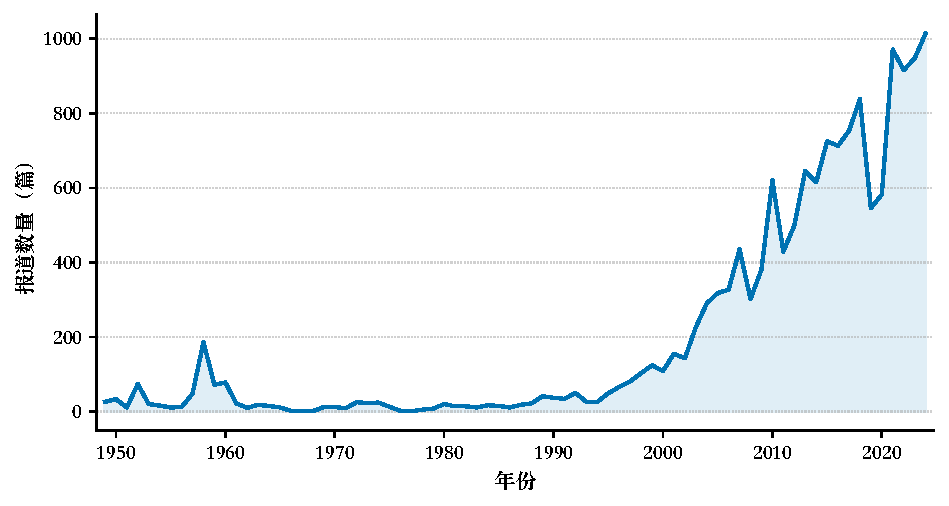
\includegraphics[width=0.85\linewidth]{charts/fig_chart1.pdf}
\par\vspace{2pt}{\small 图2-1\quad 《人民日报》环境新闻报道数量随时间发展趋势（1949—2024）}
\end{figure}

\subsubsection{二、报道体裁消息为主，通讯与评论为辅}\label{ux4e8cux62a5ux9053ux4f53ux88c1ux6d88ux606fux4e3aux4e3bux901aux8bafux4e0eux8bc4ux8bbaux4e3aux8f85}

新闻体裁能够有效反映媒体报道的框架特征、特定议题的叙事策略及其背后的传播意图。在样本中，消息这一类型共有6165篇，占比高达40.9\%，其内容篇幅短，注重时效性，主要关注环保政策公开与相关会议内容概述，这说明了主流官方媒体的主要职能，即致力于向群众及时地传递政策动态并公开环境建设信息。通讯与评论的样本量与刊登频次相近，分别为3651篇（占比24.2\%）与3128篇（占比20.8\%），深度报道共出现1246篇（占比8.27\%），科普与研究性文章为811篇（占比5.4\%），以图片为主要信息表达手段的图片新闻占比最少，只出现64篇（占比0.43\%）。（如图2-2所示）

\begin{figure}[htbp]
\centering
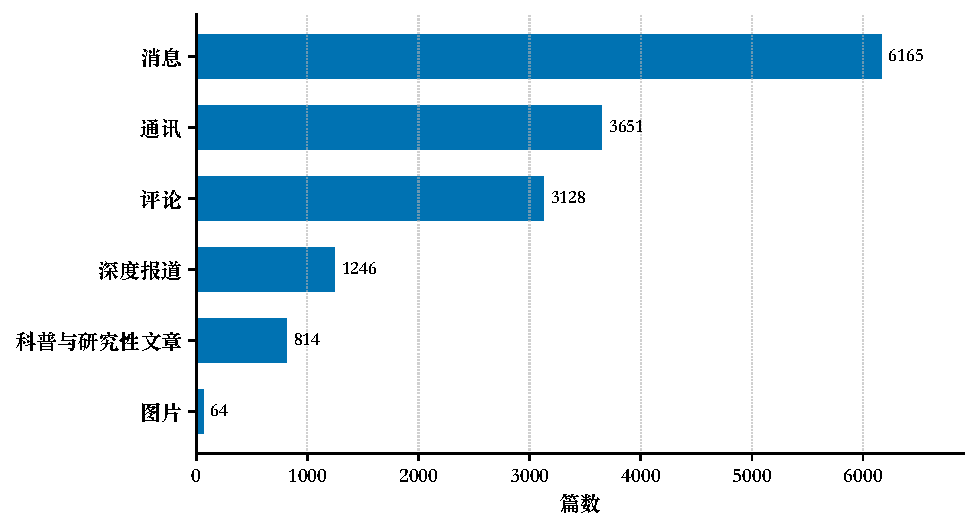
\includegraphics[width=0.8\linewidth]{charts/fig_chart2.pdf}
\par\vspace{2pt}{\small 图2-2\quad 《人民日报》环境报道体裁分布}
\end{figure}

\subsubsection{三、以官方信源作为重要参考}\label{ux4e09ux4ee5ux5b98ux65b9ux4fe1ux6e90ux4f5cux4e3aux91cdux8981ux53c2ux8003}

在信源统计中，以媒体自采自评的新闻样本最多，为6825篇（占比45.3\%）。政府信源出现频率与其相近，共有6373篇（占比42.3\%），其中涉及内容包含政府讲话、政策与制度出台等，证明了《人民日报》对于政府信息的高度依赖，体现出其跟随政府行动，注重借助政府的信源担保增加公信力和权威性。剩余报道信源在整体样本中占比偏低，从高到低依次为企业961篇（占比6.38\%）、学术界530篇（占比3.52\%）、涉及国际260篇（占比1.73\%）、普通公众94篇（占比0.62\%）、环保组织25篇（占比0.17\%）。（如图2-3所示）

\begin{figure}[htbp]
\centering
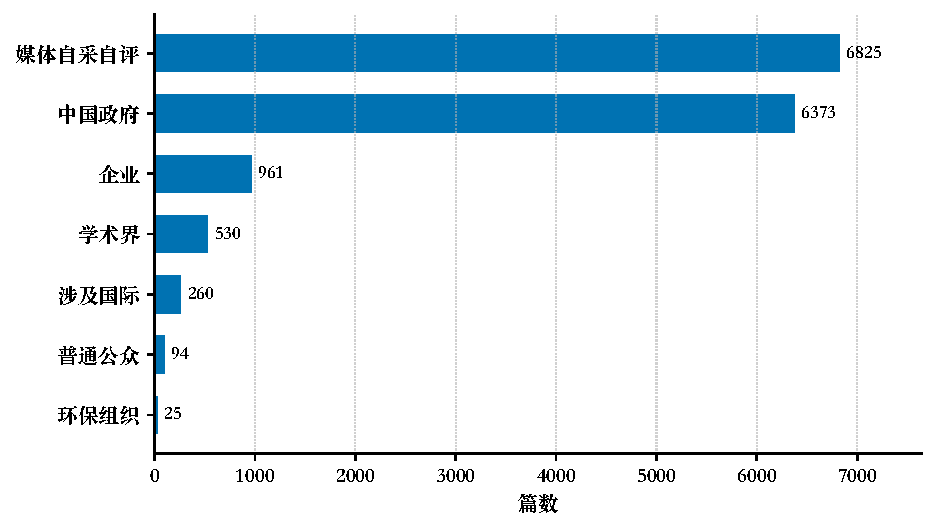
\includegraphics[width=0.8\linewidth]{charts/fig_chart3.pdf}
\par\vspace{2pt}{\small 图2-3\quad 《人民日报》环境报道信源分布}
\end{figure}

\subsubsection{四、报道议题以常规设置为主，二级议题分布显著集中}\label{ux56dbux62a5ux9053ux8baeux9898ux4ee5ux5e38ux89c4ux8bbeux7f6eux4e3aux4e3bux4e8cux7ea7ux8baeux9898ux5206ux5e03ux663eux8457ux96c6ux4e2d}

《人民日报》对环境议题的相关报道中，常规性议题报道占据了绝大多数的篇幅，其出现频次为14556篇，占到报道总数的96.6\%，远多于周期性议题的2.4\%与突发性议题的1\%。

而在细分二级议题中，前三大议题（环境政策法规25.4\%、产业优化/能源结构调整21.4\%、生态区或生物多样性15.4\%）合计占比达62.2\%，加上全球环境治理或国际合作（13\%）与水污染防治（8.83\%），前5类议题累计占比超84.3\%，二级议题分布显著集中。在二级议题``污染防治类''中，水污染防治（8.83\%）和大气污染防治（4.42\%）相对突出，而土壤污染防治（0.54\%）和重金属污染（0.05\%）占比低于其他污染防治类议题，核与辐射（0.34\%）与化学品污染（0.11\%）因其议题类型特殊受到关注较少。

经过交叉分析，我们可以观测到：在1949年---2024年的环境新闻报道中，常规性议题中出场率前三位的二级报道议题分别是``政策法规类''\,``产业优化或能源结构调整类''\,``生态区或生物多样性''，其二级报道议题分布正体现出常规环境报道议题相应内容，即对长期且持续的环境议题的关注。突发性报道议题常由``公共卫生''\,``水污染治理''\,``全球环境治理或全球合作''等二级议题构成。周期性报道议题几乎集中于``全球环境治理或全球合作''，占到了该二级议题的98\%，其常被表现为如``世界环境日''\,``世界气象日''\,``环境保护协议签订纪念日''等节日仪式性报道，通过国际间环境日的宣传，强调进行环境保护实践的主体并非被国别界限撕裂，而是整个人类群体这一事实，借此和国际主体进行互动交流。（如图2-4所示）

\begin{figure}[htbp]
\centering
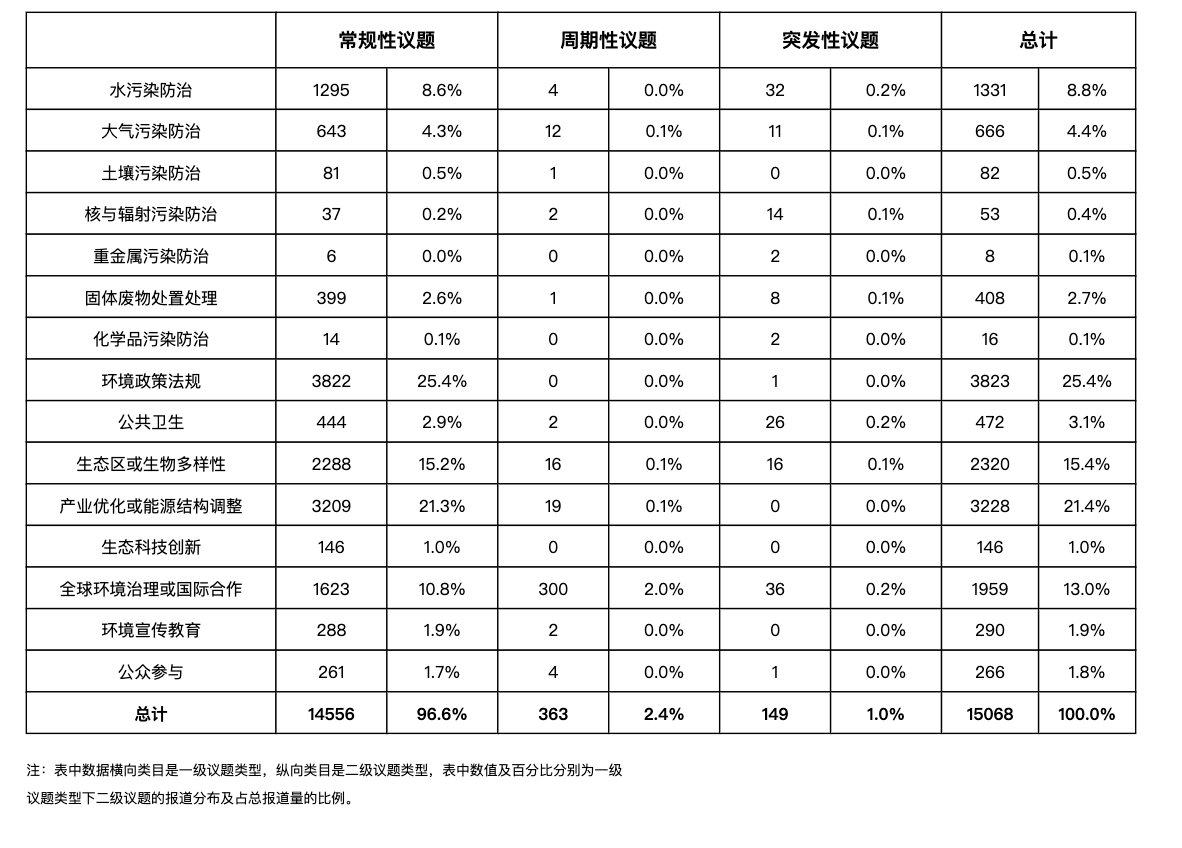
\includegraphics[width=0.8\linewidth]{media/media/image1.png}
\par\vspace{2pt}{\small 图2-4\quad 《人民日报》环境报道议题分布}
\end{figure}

\subsubsection{五、整体叙述方式偏硬，软新闻比例较低}\label{ux4e94ux6574ux4f53ux53d9ux8ff0ux65b9ux5f0fux504fux786cux8f6fux65b0ux95fbux6bd4ux4f8bux8f83ux4f4e}

在《人民日报》1949---2024年的新闻报道中，硬新闻的比例占到总体新闻量的74.4\%，软新闻为剩下的25.6\%。（如图2-5所示）硬新闻题材较为严肃，着重于思想性、指导性和知识性的新闻。\footnote{甘惜分主编.(1993).
  《新闻学大辞典》. 河南人民出版社, p.11.}而软新闻人情味较浓、写得轻松活泼，易于引起受众感官刺激和阅读视听兴趣，多着重于社会新闻书写。硬新闻的高度占比，是《人民日报》进行新闻传播活动的特征之一，映照了《人民日报》作为中共中央机关报和中心主流媒体需要进行传递政策，引导舆论，确保国家重大议程的宣传发布，维护议题权威的重要功能。《人民日报》在环境议题上保持了同其他议题一致的书写风格，多布置以思想性、指导性、知识性等需要具备一定理解能力的深度文章。

虽然在这种二元分类下，软新闻比例稍低，但其仍然体现出《人民日报》为贴近群众所作出的努力。《人民日报》在环境新闻上所呈现的``硬新闻主导、软新闻辅助''结构，是中国主流媒体平台和``喉舌''属性与大众传播规律的典型，这一平衡结构既保障了《人民日报》作为``喉舌''的权威，又通过有限但切实的软新闻增强贴近性，体现了主流媒体在环境议题上进行``舆论引导''与``发动群众''的双重逻辑。

\begin{figure}[htbp]
\centering
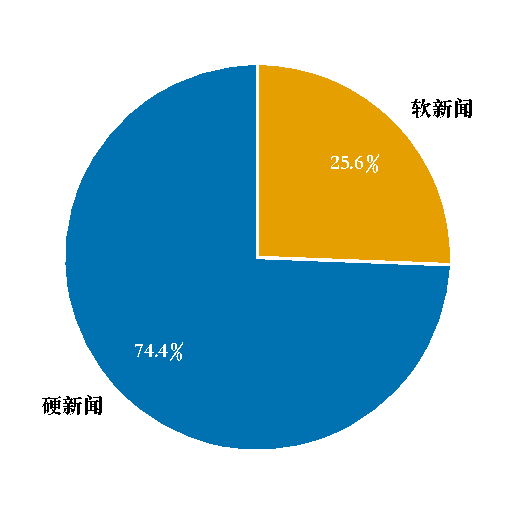
\includegraphics[width=0.55\linewidth]{charts/fig_chart4.pdf}
\par\vspace{2pt}{\small 图2-5\quad 《人民日报》环境报道软硬新闻比例}
\end{figure}

\subsubsection{六、政府作为主导地位的关涉主体，影响报道内容}\label{ux516dux653fux5e9cux4f5cux4e3aux4e3bux5bfcux5730ux4f4dux7684ux5173ux6d89ux4e3bux4f53ux5f71ux54cdux62a5ux9053ux5185ux5bb9}

文本数据显示，各类主体在《人民日报》75周年以来的环境新闻报道中出现差异显著。政府部门共出现11832次（占比79.4\%），占据主导地位。企业出现频次排名第二，共计1483次（占比9.84\%）。其后为国际主体，共计778次（占比5.16\%）。学界（424次/2.8\%）、普通公众（568次/2.04\%）和环保组织（45次/0.3\%）在整体样本中的出现频次较少，占比较低。（如图2-6所示）

结合《人民日报》所呈现的相应关涉主体的具体行为形象分析，我们可以观测到各行为主体在主流媒体中所被呈现的具体形象特征。占据最大报道篇幅的是政府群体，其形象常以``完善政策法规''\,``生态修复''\,``国际协作''\,``污染防治''的方式出现，对应监管者、督促者、协作者的正面形象，此三类在整体以政府为关涉主体的报道中占比达到83.4\%，而问责处理，承认不足的尖锐的批评与被批评者形象出现较少（合计只占比2\%）。在《人民日报》关涉的国际主体报道中，国际协作占到了其报道的绝大篇幅（占比达到91.8\%），其他行为形象频次较少，说明在报道中，国际主体常被构建为协助者的形象出现。对于企业而言，其行为形象存在正负面交织的情况：``生态修复''\,``科技创新''\,``节能减排''的正面叙述形象占到整体的94.9\%，同时也存在``违法排放''\,``遮掩问题''\,``传统产能依赖''等负面形象。对于学界而言，技术创新是其最主要的表现形式。环保组织偏向于组织活动。普通公众最常见的行为形象为环保监督和模范示例，作为环境议题的监督者和议题实践传播者出现。

\begin{figure}[htbp]
\centering
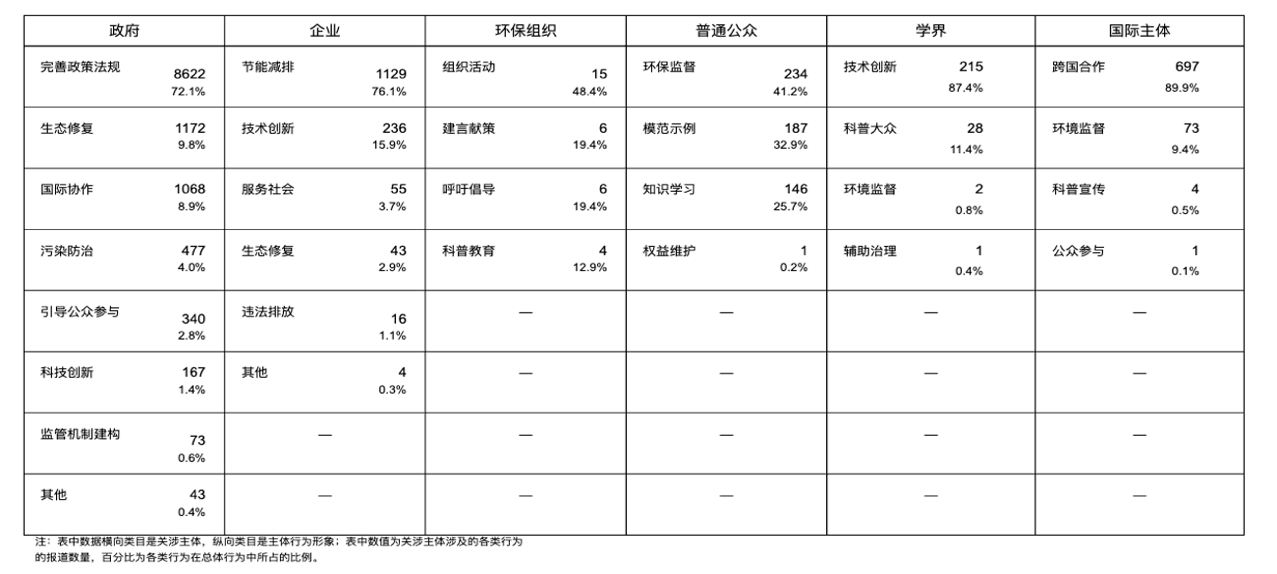
\includegraphics[width=0.8\linewidth]{media/media/image2.png}
\par\vspace{2pt}{\small 图2-6\quad 《人民日报》各信源对关涉主体的引用分布}
\end{figure}

\subsubsection{七、整体偏向积极报道，情感倾向在后期呈现两极分化}\label{ux4e03ux6574ux4f53ux504fux5411ux79efux6781ux62a5ux9053ux60c5ux611fux503eux5411ux5728ux540eux671fux5448ux73b0ux4e24ux6781ux5206ux5316}

在全样本中，积极类报道占绝对主要地位，共计12945篇（占比85.9\%），倾向中立的报道共计1940篇（占比12.9\%），消极类倾向报道共计183篇（占比1.21\%）。这体现了《人民日报》在环境相关议题上呈现出积极向上的报道面貌，反映出主流媒体在引导社会正向氛围的贡献和努力，同其社会主流媒体的定位相吻合。

在对报道情感倾向和关涉主体进行交叉分析后，我们发现作为《人民日报》主要关注的政府主体相关报道中，积极情感倾向报道占到整体积极报道的79.4\%，而在所有关涉政府的新闻报道中，积极情感倾向占到87.1\%。在为数不多的消极情感倾向报道中，所涉及的主体最多为政府和国际主体。（如表2-1所示）在历时性上，报道情感倾向在1972年后存在明显的两极分化趋势，即其在环境议题上的新闻报道随时间变迁，显得愈发积极。（如图2-7所示）

\begin{longtable}[]{@{}
  >{\centering\arraybackslash}p{(\linewidth - 8\tabcolsep) * \real{0.1968}}
  >{\centering\arraybackslash}p{(\linewidth - 8\tabcolsep) * \real{0.2142}}
  >{\centering\arraybackslash}p{(\linewidth - 8\tabcolsep) * \real{0.2142}}
  >{\centering\arraybackslash}p{(\linewidth - 8\tabcolsep) * \real{0.1965}}
  >{\centering\arraybackslash}p{(\linewidth - 8\tabcolsep) * \real{0.1785}}@{}}
\toprule\noalign{}
\begin{minipage}[b]{\linewidth}\centering
\end{minipage} & \begin{minipage}[b]{\linewidth}\centering
中立
\end{minipage} & \begin{minipage}[b]{\linewidth}\centering
消极
\end{minipage} & \begin{minipage}[b]{\linewidth}\centering
积极
\end{minipage} & \begin{minipage}[b]{\linewidth}\centering
总计
\end{minipage} \\
\midrule\noalign{}
\endhead
\bottomrule\noalign{}
\endlastfoot
政府 & 1448

9.6\% & 91

0.6\% & 10423

69.2\% & 11962

79.4\% \\
企业 & 74

0.5\% & 10

0.1\% & 1399

9.3\% & 1483

9.8\% \\
国际主体 & 251

1.7\% & 55

0.4\% & 472

3.1\% & 778

5.2\% \\
学界 & 84

0.6\% & 2

0.0\% & 160

1.1\% & 246

1.6\% \\
普通公众 & 77

0.5\% & 232

0.2\% & 468

3.1\% & 568

3.8\% \\
环保组织 & 6

0.0\% & 2

0.0\% & 23

0.2\% & 31

0.2\% \\
共计 & 1950

100\% & 183

100\% & 12945

100\% & 15058

100\% \\
\end{longtable}

\begin{center}
表2-1
\end{center}

\noindent 注：表内数据横向类目是各主体的态度，纵向类目是关涉主体；表内数值为特定信息来源对变量主体的引用数量统计；百分比为各单元格数据占总体的百分比。

\begin{figure}[htbp]
\centering
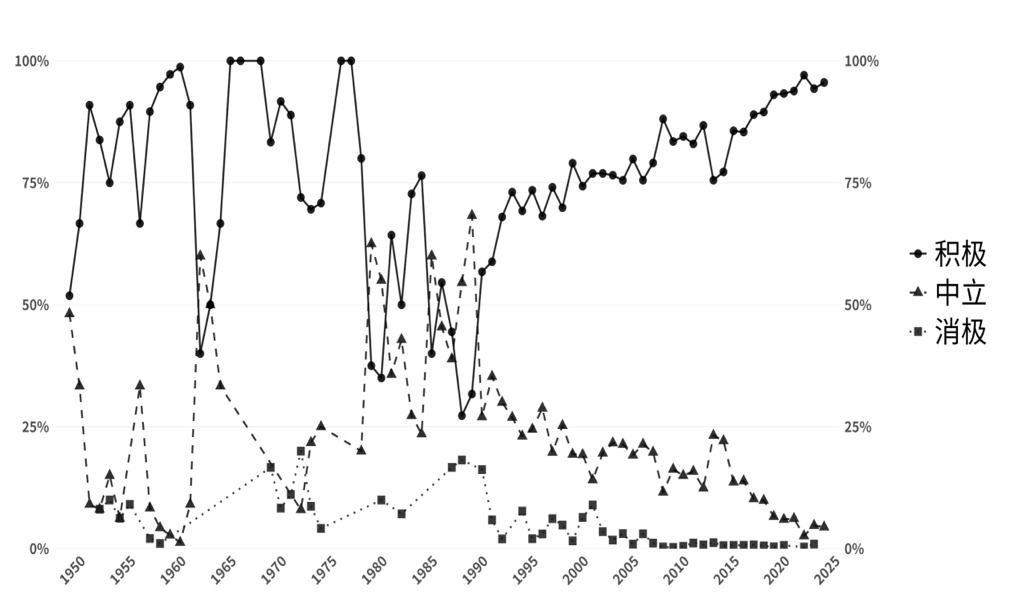
\includegraphics[width=0.8\linewidth]{media/media/image3.png}
\par\vspace{2pt}{\small 图2-7\quad 《人民日报》环境报道情感倾向交叉分析}
\end{figure}

\subsection{第四节
《人民日报》环境新闻的报道框架与话语实践}\label{ux7b2cux56dbux8282-ux4ebaux6c11ux65e5ux62a5ux73afux5883ux65b0ux95fbux7684ux62a5ux9053ux6846ux67b6ux4e0eux8bddux8bedux5b9eux8df5}

早在1974年，戈夫曼便指出框架的存在能够有助于人们在所处的混乱无序的社会中快速地寻找、感知，甚至标签化人们想要获取的事件和信息。由此，框架分析（Framing
Analysis）被引入到社会科学研究领域之中，而在传播内容研究领域，框架分析则被发展成为一种研究新闻文本的方法。

媒体框架以前后一致的方式来对新闻事件做出选择、强调和排除，使得对事件的某些理解在文本里更加突出，并且成为受众感知到的社会真实。\footnote{陈阳.
  (2007). 框架分析:一个亟待澄清的理论概念. 《国际新闻界》, (04),
  19-23.pp.20-21.}在一定程度上而言，费尔克劳（Norman
Fairclough）的宏观命题话语分析和由戈夫曼（Erving
Goffman）等学者推动形成的媒介框架研究存在相通之处，即都将关注点放置于媒介的生产环节，通过此类框架分析，可以认知到新闻文本如何被生产出来，又如何被受众消费与解读\footnote{何威,曹书乐.
  (2018).
  从``电子海洛因''到``中国创造'':《人民日报》游戏报道(1981-2017)的话语变迁.国际新闻界,40(05),57-81,p.68.}，从而从宏观话语命题层面解读环境传播话语的整体设置布局。

前文展示了《人民日报》新中国成立后环境新闻文本的整体发展态势，接下来本节将基于对《人民日报》在环境议题上的梳理，并参考李娜、朱乙等学者的研究成果，将《人民日报》展现的报道框架分为``制度理性框架''\,``生态文明框架''\,``国家叙事框架''\,``技术赋能框架''\,``经济争夺框架''\,``风险对抗框架''共六种，用以对样本进行归纳分类和宏观话语命题分析，研究主流媒体如何设计并运用报道框架来引导环境新闻走向，进而引导受众的认知与态度。

\subsubsection{一、环境报道六大框架及宏观话题实例}\label{ux4e00ux73afux5883ux62a5ux9053ux516dux5927ux6846ux67b6ux53caux5b8fux89c2ux8bddux9898ux5b9eux4f8b}

（一）制度理性框架：将政治话语转化为新闻话语

制度理性框架把环境专业话语、法制话语、学术话语、管理话语、理论话语转化为公共传播话语，展现国家出台相关环境的政策法规、研究成果、惩治进程\footnote{李娜.
  (2019). 从爱国到文明:建国70年主流媒体环境话语变迁与共意动员. 新闻界,
  12,38-49,p.43.}，此报道框架所设计的新闻内容通常强调通过建立和完善法律法规，规划和改善行政管理体系来应对环境挑战。报道主要关涉主体为政府，并说明政府如何通过制度化的手段来管制、协调社会间各行为主体的行动，以达到环境保护的目标。如《人民日报》发布的《环保督查直指地方保护热点解读》（2006年12月6日），就将全国各级省市环保督查中心的揭牌、职责内容、设置原因进行了解读，并着重点出国家意志在进行环境保护行动的坚决，为典型的制度理性框架报道。同月22日发表的《促进人与自然和谐的几个问题》（2006年12月22日）则以学界的理论视角点出了进行环境保护的紧迫性以及其对当代经济发展和可持续发展的必要性，说明``人与自然和谐''是``社会主义和谐社会''的重要内容，由此进行国家环境保护意志的公共化撒播，也是制度理性框架的表达特征。

（二）生态文明框架：将环境保护和文明形态结合

此报道框架主张将环境保护建构为先进文明形态的内核之一，通过对环境保护实践行为和典型人物案例的报道，强调以``环保''为文明，并用中国式现代化和``美丽中国建设''等宏观叙事对其进行接洽。《周庄人与水的协奏曲建设》（2006年4月27日）一文就以积极的报道态度对江苏省昆山市周庄镇的环境建设成果做了展示，意在将其打造为乡镇环境建设样板间，促进生态文明建设话语。典型框架同样可见《环保与和平》（2004年10月24日），一篇描述以该年获诺贝尔和平奖的环保主义者马塔伊博士为描写中心的人物文章------同样通过典型人物的树立宣传环境保护话语，并由此将``环境保护''同``和平''\,``和谐共生''\,``宽容博爱''等与先进文明所关涉的语词与内涵进行结合，塑造出进行环境保护建设的行为先进性。

（三）国家叙事框架：对外进行批评或斗争

该框架将环境议题编织进宏大的国家建设活动或国际关系互动之中，意在利用环境议题来塑造国家形象，凝聚国民认同，以环境议题为抓手，同各国际主体进行互动，或批评，或赞扬他国成就，或强调人类命运共同体进行联合环保实践。在这个框架下，环境报道不只是环境报道，而被赋予了超越环境本身的国家意义。在《人民日报》早期的环境报道中，该种报道框架常常被作为具有攻击性的国际话语武器------如谴责美方发动细菌战、指出资本主义国家的工业污染并同我国环境建设成果进行比对，以1969年发表的评论文章《瘟神装不成菩萨》（1969年）为典型性代表。但随着我国逐渐嵌入世界环境保护运动体系之中后，国家叙事框架就开始逐渐偏向于强调国际环境事务合作或周期性的国际环境保护活动报道，如《在中美环境与发展讨论会上的讲话》（1997年3月26日）与《让清洁美丽世界为文明添彩》（2017年11月21日）。但同时对于国际主体的反环境保护举动仍具备批评作用。

（四）技术赋能框架：技术即通向环境保护的出路

该报道框架强调将科技创新和应用视为解决环境污染问题的关键驱动力或主要途径，主张通过技术来协调人与自然的关系，聚焦于发展清洁技术、改造传统污染产业、加强环境监测等新闻事件。较为典型的报道有《垃圾、污水、污泥的肥份》（1959年1月26日）、《洒水控粉尘植树绿荒山》（1999年7月21日）、《适度发展核电是正确选择》（2001年4月26日）、《一家绿色工厂的升级之路》（2023年3月30日）。其内容涉及逐渐由初期的环境资源利用科普转向以技术为主要核心的环境保护发展道路。

（五）经济争夺框架：经济发展与环境保护的辩证关系

该框架聚焦于环境与经济活动的相互影响和联系，探讨两者在发展之际的矛盾冲突以及协调发展路径。其既关注环境保护行动对经济增长、产业结构调整以及就业等方面带来的挑战与代价，也关注生态改善和绿色产业带来的新型价值与长远的经济效益。《环境污染------人类的慢性自杀》（2001年9月6日）就报道水污染对于渔业生产经济的破坏以及对渔民、农民的生存状况影响问题，重点指出水污染往往来源于地方支柱产业，揭示出经济发展与环境保护之间的矛盾点。《排污``假方案''何日成历史》（2004年10月21日）以武汉钢铁（集团）公司为例，指出经济发展与环境保护处理成本之间的抉择困境，并以岳阳纸业股份有限公司在改造设备的投入、环境保护具体的成效以及循环经济发展实践，为企业经济生产和环境保护之间提供协调路径。

（六）风险对抗框架

该框架会将环境问题建构为对国内以及国际社会发展具有阻碍的风险或危机，并说明其对人类可持续发展的现实性或潜在性的威胁，通过说明克服环境问题的举措进行叙事，或者陈述问题营造出紧迫的氛围，从而突出环境保护实践的紧迫。此框架的典型报道《广东贵屿：为电子垃圾污染敲响警钟》（2004年5月17日）便从广东贵屿的电子垃圾拆解与处理问题出发，由国内环境问题延展到国际问题，从而将电子垃圾这一环境保护子问题的现实紧迫性进行了突出。

\subsubsection{二、《人民日报》环境新闻报道框架呈现}\label{ux4e8cux4ebaux6c11ux65e5ux62a5ux73afux5883ux65b0ux95fbux62a5ux9053ux6846ux67b6ux5448ux73b0}

经过描述性数据分析可以发现，制度理性框架在整体框架布局中占据了绝大部分，频次为7961次，占比最高。紧随其后的是生态文明框架，频次为3669次。相对而言，技术赋能框架和国家叙事框架的出现频次较少，分别为1631次和1421次。经济争夺框架和风险对抗框架是出现频次最少的框架，分别为269次和117次。《人民日报》在环境新闻报道上的总体布局呈现出不均衡的状态，制度理性框架和生态文明框架在整体报道中占据了主导地位。而这也正符合主流媒体状态，在环境传播议题选择与建构上存在的具有天然倾向的表达。（如表2-2）

\begin{longtable}[]{@{}
  >{\centering\arraybackslash}p{(\linewidth - 4\tabcolsep) * \real{0.3327}}
  >{\centering\arraybackslash}p{(\linewidth - 4\tabcolsep) * \real{0.3146}}
  >{\centering\arraybackslash}p{(\linewidth - 4\tabcolsep) * \real{0.3527}}@{}}
\toprule\noalign{}
\begin{minipage}[b]{\linewidth}\centering
框架名称
\end{minipage} & \begin{minipage}[b]{\linewidth}\centering
数量
\end{minipage} & \begin{minipage}[b]{\linewidth}\centering
占比
\end{minipage} \\
\midrule\noalign{}
\endhead
\bottomrule\noalign{}
\endlastfoot
制度理性框架 & 7961 & 52.8\% \\
生态文明框架 & 3669 & 24.3\% \\
技术赋能框架 & 1631 & 10.8\% \\
国家叙事框架 & 1421 & 9.43\% \\
经济争夺框架 & 269 & 1.79\% \\
风险对抗框架 & 117 & 0.78\% \\
\end{longtable}

\begin{center}
表2-2
\end{center}

从数据来看，制度理性框架几乎贯穿了所有年份，并且在各个时期的报道中长期占据最高频次。在2010年之后，其年均出现数量逐年上升，占年度环境新闻报道比例呈波动上升。生态文明框架自2000年起，尤其在2010年以后，逐渐得到较多应用。2020年后，其在报道中的出现频次显著增加，反映出全球环保议题和可持续发展目标的加强，生态文明框架逐渐成为环境报道中的重要组成部分。技术赋能框架在2010年代开始得到更多的关注，随着现代中国技术社会的推进与绿色中国的倡议提出，技术赋能框架逐渐呈现增长趋势。（如图2-8所示）国家叙事框架虽然在总体上不如制度理性框架和生态文明框架频繁使用，但其在一些关键时期逐步增加，特别是在国家战略、国际关系以及国内重大政策变动期间，体现了国家层面叙事的权重。经济争夺框架和风险对抗框架的使用频率波动较大，整体较低。这两个框架通常在经济危机、重大风险事件或突发性问题报道中出现，具有较强的时效性。

\begin{figure}[htbp]
\centering
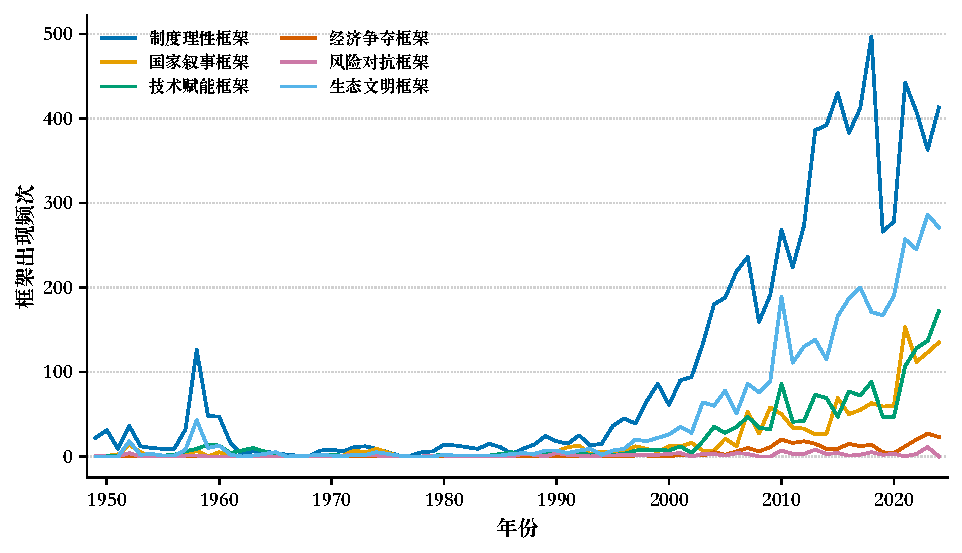
\includegraphics[width=0.9\linewidth]{charts/fig_chart5.pdf}
\par\vspace{2pt}{\small 图2-8\quad 《人民日报》环境报道六大框架逐年分布}
\end{figure}

\subsubsection{三、《人民日报》环境报道的话语实践}\label{ux4e09ux4ebaux6c11ux65e5ux62a5ux73afux5883ux62a5ux9053ux7684ux8bddux8bedux5b9eux8df5}

``环境''的意义并非静态的，稳定的，固定的，而是作为文化或政治的构造物出场的，或者说，``环境''的意义是被建构的、被发明的、被争夺的。\footnote{刘涛.
  (2011). 《环境传播：话语、修辞与政治》. 北京大学出版社, pp.9-10.}费尔克劳认为，话语能够再现物质世界的过程、关系和结构，也投射、想象和再现不同于现实世界的可能世界。\footnote{诺曼·菲尔克劳夫.
  (2023). 《话语分析 社会科学研究的文本分析方法》. 商务印书馆, p.146.}要研究主流媒体环境新闻话语的具体流变，并解释其如何被形构或决定的，就必须探讨文本内容和背后权利关系的相互作用。黄河认为，《人民日报》的环境新闻议题的建构规律，核心线索在于其对政府议程的跟随，并受其主导呈现出报道议题选择的``偏向性''和属性叙事的``非问题化''。\footnote{黄河.
  (2022).
  《走向和谐共生：中国环境议题的多元话语建构》（新闻传播学文库）.中国人民大学出版社,
  p.74.}可以认为，《人民日报》的新闻文本是政治和政府社会实践的情景化转化，同时也在情景化过程中向大众传播，融入不同社会实践的文本和互动之中。根据前文内容分析梳理，我们也不难发现，以《人民日报》为代表的主流媒体在议题、关涉主体、信源等新闻生产流程上，都与政府时时靠近，时时受其影响，并将政府议程传递至其他社会文本，由此影响社会实践。因此，如果要对《人民日报》所传播的环境新闻文本进行话语分析，就无可避免地需要下沉到中国新中国成立以来关于``环境''的社会文化实践，特别是在政府指引下的社会文化实践之中。

下列段落将根据《人民日报》新中国成立75周年来环境新闻的文本报道特征变化情况以及从政府环境工作实践视角折射出的中国社会环境保护观念史，将1949年至2024年划分为四个历史时期，展现《人民日报》环境新闻的话语流变过程。

\textbf{（一）话语建构之初：作为``公共卫生''的环境保护（1949-1972）}

在1949---1972年间，国家还处于生产生活物资较为匮乏的阶段，需对自然环境进行大力开发，以满足对生活生产资料补给的需求，社会以积极拓荒、开发环境进行经济建设为风气。因而这一时期，对于环境的保护并尚未被纳入国家治理范畴之内，而是被排除在主流话语之外------环境保护''一词尚未具备现代意义上的生态保护与污染防治实践相关联，而只是被视作公共卫生保护活动与经济活动的子命题。在特殊时期，也会被当作用来辅助军事和政治进行意识形态对抗的话语武器，如批驳``美帝国主义''的``细菌战行径''，也有以1971年3月11日消息文章《美国社会危机日益深化》为典型代表，通过揭露西方工业生产对环境破坏现实以批驳资本主义制度的类型文章。

内容分析可见，《人民日报》在这一时期内``公共卫生''的二级议题报道共出现449篇，占到这一时期环境新闻报道总量的61.9\%，其报道形式以消息类和深度报道类为主。该时期《人民日报》将环境新闻报道议题集中于公共卫生范畴，其``环境''概念尚未拓展至生态保护或生物多样性领域，而更多聚焦于群众生活和生产空间的卫生治理，注重其在建设``文明社会''的重要表征作用。如1949年10月29日出现的第一篇环境新闻《预防鼠疫侵袭首都》就倡导通过进行环境卫生清洁，以抗击疫病的扩大传播。1952年8月30日刊登的《爱国卫生运动逐步深入广大农村》展示了一系列的环境卫生清洁工作开展先进的乡镇，具象化呈现``粪便管理''\,``灭蝇捕鼠''\,``清洁猪牛栏''等措施如何``增加肥料''\,``提高产量''\,``防范疾病''\,``降低死亡率''。其报道设置的核心目的，在于跟随政府的发展意图，通过报道``环境卫生建设''来对群众进行相应指导，将``环境卫生''建构为影响社会文明程度与生产生活质量的重大指标，由此保障公众健康，推动生产有序发展。因其具体历史情景，``环境保护''所关涉的语词意义还较为单薄，距离当下所言的``环境保护''还存在巨大的填充空间。

\textbf{（二）边缘到中心：以``法制筑基''的环境保护（1972-2002）}

1972年6月，中国派出代表参加联合国在斯德哥尔摩召开的第一次人类环境会议，环境保护和经济社会发展的相关联系被政府重新考量。会后，中国开始建立环保机构，着手工业``三废''（废水、废气和固体废物）的防治与环境规划。\footnote{张坤民,温宗国,彭立颖.
  (2007). 中国的环境政策:形成、特点与评价. 中国人口·资源与环境,
  2,1-7,p.1.}1973年8月，第一次全国环境保护会议在北京召开，会议通过了《关于保护和改善环境的若干规定（试行）》，中国当代的环境保护与环境治理实践正式开始。面对国内的``环境保护''这一语词内涵的空乏与群众对于``环境保护实践''的认知缺失，政府单位通过一系列的会议商讨，出台政策法规，设置管理机构，初步确定了``环境保护''应当保护什么，应当如何保护，为今日对于``环境保护''的言谈提供了基础。这种探索的过程，在同期《人民日报》的新闻报道中能得到鲜明体现。

在这一时期，通讯、评论、深度文章以及科普和研究性文章的比例迅速上升，消息体裁由1949---1972年间的62.9\%占比下降到41.8\%。主流媒体的环境新闻议题，开始由简单快速的消息引介和传达，向有深度、有思考的文章进行转向。同时，在报道倾向层面，相关环境新闻的情感表达更加丰富，积极情感倾向报道由上个时期的86.2\%下降到68.8\%，消极情感倾向和中立情感倾向报道数量迅速增加。相较于早期环境新闻在涉及国际主体时的批驳，国际主体由以往的``破坏者''向``先进参考者''迈进，如1979年1月4日第六版的《日本环境保护的成就是怎样取得的》，通过介绍中国环境代表团在日本考察的所见所闻，介绍环境保护的先进经验。在国内层面，面对``环境保护''这一语词内涵的空乏与群众对于``环境保护实践''的认知缺失，由政府主导的话语开始下沉，其内涵开始逐渐突破上个时期较为单调的``环境卫生''框架的限制，得到充实。例如，1983年底召开的第二次全国环保会议，会上提出将环境保护上升到基本国策，明确了环境保护在中国经济社会发展中的重要地位。

在1972---2002年的三十年间，``政策法规''一直是《人民日报》环境新闻报道的主要二级议题，占比达到全部二级议题的29.1\%，每当政府对重要的环境政策进行讨论或者发布重要的环境政策法规，《人民日报》便会进行跟进报道。例如，1990年12月15日发表的消息《国务院关于进一步加强环境保护工作的决定》以及1991年6月4日对国家环境保护局发布当年环境状况公报的行动等诸多类型文章。就这一时期的新闻文本特征和内容表现而言，环境议题呈现出一种显然的由边缘走向中心的趋势。

\textbf{（三）管制到疏导：以``技术为核''的环境保护（2003-2012）}

西蒙栋曾在《技术对象的存在方式》中指出：技术对象是人类活动的结晶，也是文化意义的表达，其能够通过协调文化及其所表达和支配的现实，为文化带来一种统一及稳定的力量。\footnote{吉尔贝·西蒙东.
  (2024). 《论技术物的存在模式》. 南京大学出版社,pp.4-7.}技术通过想象在主体与客体、物质与符号之间建立动态中介，其既是社会话语的物化，也是社会实践的载体，技术实践出的实际效用会在一定程度上形成对社会话语的补正。技术想象不仅具象化于技术本身，而且存在于技术所创造的社会规范和文化实践中。有时，技术想象捍卫和加强社会与文化现状；有时，它们的存在成为打破稳定系统的``熵''。\footnote{徐旭,陈凡.
  (2021).
  技术想象：技术创新和发明应用的核心------第22届国际技术哲学学会(SPT)会议述评.
  哲学分析, 12(06),179-189,p.180.}

2003年7月28日，胡锦涛在讲话中提出科学发展观，宣扬``坚持以人为本、树立全面协调可持续的发展观''，统筹人与自然和谐发展，把人和环境的关系高度绑定起来，强调发展不应以牺牲环境为代价，而是应该以``可持续''为目标对生产生活实践进行审视，并对生态环境进行维护管理。在政府的话语号召与前期国际环境保护交流经验影响下，我国对于环境保护的方法论认识，逐渐由法律法规管控的``压制性''保护方法上升到以技术为核心的``疏导性''保护方法，技术在政治议题中被更高频次地提及，技术以一种强而有力的工具姿态进入到环境议题中。

通过分析不同时期的二级议题词频，我们可以清晰地观察到，从2003年开始，产业优化或能源结构类议题调整一跃成为出现频次最高的二级议题。相比于1949---1972年的3.6\%占比和1973年---2002年的6.6\%占比，在这一时期，该议题共有1155篇，占该时期总体环境新闻报道的30.2\%------在数量和占比上均实现了显著的增长；技术赋能类框架也在彼时迎来飞速发展。以学术界和企业为信源的稿件频次上升到第三位和第四位。同时，环境新闻的数量迎来了大幅增长，较1973---2002间的1250篇，增长到了3827篇；但就情感倾向而言，消极倾向报道数量有所降低，中立和积极报道占比较往期比例上升。

以``科学''的姿态对待环境保护，以技术为推动来解决环境问题，以期可持续发展成为这一时期社会主导的话语风向。马华芳对这一时期《人民日报》关于``垃圾处理''这一细分议题报道进行了分析思考，发现这一时期上出现了大量讨论科学处理垃圾、提高垃圾处理技术、介绍国外先进技术的新闻报道。\footnote{马华芳.
  (2020). 环境传播视域下主流媒体关于垃圾议题报道的话语变迁.
  华中师范大学,1-49.pp.34-36.}。清洁生产技术、治理污染技术、改善生态技术和新能源技术等具体的生态化科技成果展示和引介，成为这一时期新闻报道的重要叙述表现手段。如2004年6月8日发表的消息稿件《让新技术好花常开》一文强调了技术在推进节能减耗的重要作用，并展示了中国节能投资公司作为政策性投资机构的投资意向和具体成果。

综合而言，在这一时期内，技术对环境所具有的工具性改造效果被政府重视起来，一定程度上将环境议题的解决方法由``管控型''转向``疏导型''。以《人民日报》为代表的主流媒体，通过新闻话语引导，潜在地将``环保议题''转化为``技术发展议题''，缓解了社会对于``环境破坏''的道德性压力，转而将焦点引向发展技术的动力，对技术的期待与对技术可能性的想象经由主流新闻媒体向下传递，在社会整体层面营造出了一种以``环保问题''为议题的技术想象氛围，将技术想象氛围深层次地嵌入了今后对于环境保护议题的讨论范畴。

\textbf{（四）改革与突破：以``共治为目标''的环境保护（2013-2024）}

顺着《人民日报》对于重大环境相关政治议题报道的脉络，我们并不难发现，``环境议题''在这一时期有了更新的变化。在2013年党的十八大上，政府将生态文明建设纳入中国特色社会主义事业``五位一体''布局，将``环境保护''提高到了最为中心的层次。习近平在2013年作出明确指示：``我们既要绿水青山，也要金山银山。宁要绿水青山，不要金山银山''，对于经济发展和环境保护的关系问题作出了突破性的回答，寓意着国家主流意识形态对环境保护的关切和认同达到了前所未有的高度。\footnote{刘琳琳,黄河.
  (2022). 新中国成立以来政府环境治理话语的演变与发展. 国际新闻界,
  44(02),58-77,p.69.}次年，新环境保护法出台，增加了公众参与、环境监督、公益诉讼等新的制度，将``全民环保''的概念融入法治文化。2020年9月，双碳目标的提出显示出一种国家层面的``外律''，并在后续的全国碳排放交易市场建设和垃圾分类管理实践中，体现出将环境保护逻辑融入到经济发展逻辑和社会生活逻辑的趋势。

这一时期，环境新闻数量迎来显著提升，十二年间年均报道数量9266篇，相比上个周期，年均新闻报道增加499篇，报道数量超过以往环境新闻总和。与此同时，软新闻在整体占比呈现波动上升趋势，《人民日报》的传播策略在长期的传播实践中逐渐发生变化，由较为硬核的政治宣导转向情感叙事，意在通过转化叙事方式对大众进行一定的情感动员。如2020年12月28日通讯文章《长江货轮船长眼里的绿色发展》，此类通过展现群众视角来进行微观叙事的多篇文章为这一时期的典型代表，其意在通过此类方式从而激发群众对环境议题的关注与行动热情。在报道议题上，环境政策法规类和产业优化或结构调整类议题占据前两位，占总体新闻报道的47.8\%，其报道重心从强调技术力量转向社会文化层面的深入探讨。这表明国家不仅通过政策引导和技术创新推进环保，也通过文化建设和社会动员促进大众环保意识的提升。

总的来说，2013年至2024年期间，《人民日报》在环境新闻话语上的转型，展现了中国社会在环境保护领域中不断深入与转向。政府由规制话语、科学话语为主向多元话语大融合转变。\footnote{黄河.
  (2022).
  《走向和谐共生：中国环境议题的多元话语建构》(新闻传播学文库).中国人民大学出版社,p.43.}《人民日报》所传递的话语观念，从起初的政策导向到后来的技术驱动，再到现在的全社会共治与绿色发展。环境新闻在表达类目和框架上的转变，承接了政府所给予的角色，就信息发射端层面，完成了话语的传递作用。

\subsection{第五节
新媒体时代主流媒体环境报道话语建构的革新与转变------以《人民日报》官方微博为例}\label{ux7b2cux4e94ux8282-ux65b0ux5a92ux4f53ux65f6ux4ee3ux4e3bux6d41ux5a92ux4f53ux73afux5883ux62a5ux9053ux8bddux8bedux5efaux6784ux7684ux9769ux65b0ux4e0eux8f6cux53d8ux4ee5ux4ebaux6c11ux65e5ux62a5ux5b98ux65b9ux5faeux535aux4e3aux4f8b}

随着媒介技术的更迭，主流媒介的话语表达方式已从传统纸媒超脱出来转向互联网------通过媒介融合的手段打造新型主流媒体，建构新型话语传播体制进行环境传播在当下成为主流媒体进行环境话语建构的重要方法，相较于传统纸媒在环境传播领域自上而下的撒播特征，新媒体表现出自下而上和横向并行的特征。\footnote{黄河,刘琳琳.
  (2014).
  环境议题的传播现状与优化路径------基于传统媒体和新媒体的比较分析.
  国际新闻界, 36(01),90-102,pp.95-98.}在漫长75周年的末端，在当下的互联网传播时代，《人民日报》如何以新的传播手段延续中国环境话语建构，也是仍需描述的问题。

《人民日报》自2012年7月开通微博客户端，良好运营至今，现已积攒1.56亿粉丝，相较于其他各大主流媒体，仍具有强大影响力与代表作用。为了深入理解主流媒体如何适应媒介环境的变化，如何在新媒体平台上延续和建构环境话语，辅助中国主流媒体环境话语的整体形成，本文接下来将以《人民日报》微博端作为主流媒体在新媒体时代的代表，对《人民日报》微博端环境新闻报道的整体文本特征以及其话语实践方式相较于其纸面报道的相似与不同，做一些简略的分析和梳理。

基于此，本文将样本数据时间段定为2012年8月1日至2024年12月31日，通过爬虫技术对《人民日报》微博数据进行了批量采集。在使用``生态''\,``环境''\,``绿色''\,``资源''\,``污染''\,``碳中和''\,``气候''等环境报道相关关键词对收集数据集进行初步检索排除后，结合具体内容上下文信息进行二次人工筛选，剔除与环境话题无关联的微博内容，最终确定《人民日报》发布的1649条环境报道作为编码与分析样本。

在文本分析方法上，此板块借鉴先前纸面新闻话语分析类目，构建``词频分布''\,``情感倾向''\,``议题类型''三类变量，对收集数据进行了编码处理。

\subsubsection{一、《人民日报》官方微博环境报道的内容呈现与分析}\label{ux4e00ux4ebaux6c11ux65e5ux62a5ux5b98ux65b9ux5faeux535aux73afux5883ux62a5ux9053ux7684ux5185ux5bb9ux5448ux73b0ux4e0eux5206ux6790}

（一）环境研究报道词频

词频能够帮助人们辨别最基本的语言特征，这些特征往往包含话语的意义。\footnote{钱毓芳.
  (2010). 语料库与批判话语分析.
  外语教学与研究,42(03),198-202+241，pp.198-199.}而词汇的选择能体现文本生产者的立场、态度及价值观念等内容，媒体通常采用不同的词汇选择策略传播特定的意识形态。如表2-3所示，本文通过统计分析得到了《人民日报》微博客户端在环境报道议题上使用的较多的30个关键词。

\begin{longtable}[]{@{}
  >{\centering\arraybackslash}p{(\linewidth - 16\tabcolsep) * \real{0.0845}}
  >{\centering\arraybackslash}p{(\linewidth - 16\tabcolsep) * \real{0.1520}}
  >{\centering\arraybackslash}p{(\linewidth - 16\tabcolsep) * \real{0.0849}}
  >{\centering\arraybackslash}p{(\linewidth - 16\tabcolsep) * \real{0.0851}}
  >{\centering\arraybackslash}p{(\linewidth - 16\tabcolsep) * \real{0.1347}}
  >{\centering\arraybackslash}p{(\linewidth - 16\tabcolsep) * \real{0.1014}}
  >{\centering\arraybackslash}p{(\linewidth - 16\tabcolsep) * \real{0.1014}}
  >{\centering\arraybackslash}p{(\linewidth - 16\tabcolsep) * \real{0.1533}}
  >{\centering\arraybackslash}p{(\linewidth - 16\tabcolsep) * \real{0.1028}}@{}}
\toprule\noalign{}
\begin{minipage}[b]{\linewidth}\centering
序号
\end{minipage} & \begin{minipage}[b]{\linewidth}\centering
关键词
\end{minipage} & \begin{minipage}[b]{\linewidth}\centering
词频
\end{minipage} & \begin{minipage}[b]{\linewidth}\centering
序号
\end{minipage} & \begin{minipage}[b]{\linewidth}\centering
关键词
\end{minipage} & \begin{minipage}[b]{\linewidth}\centering
词频
\end{minipage} & \begin{minipage}[b]{\linewidth}\centering
序号
\end{minipage} & \begin{minipage}[b]{\linewidth}\centering
关键词
\end{minipage} & \begin{minipage}[b]{\linewidth}\centering
词频
\end{minipage} \\
\midrule\noalign{}
\endhead
\bottomrule\noalign{}
\endlastfoot
1 & 中国 & 607 & 11 & 垃圾 & 298 & 21 & 国际 & 176 \\
2 & 视频 & 496 & 12 & 世界 & 256 & 22 & 人民 & 161 \\
3 & 人民日报 & 406 & 13 & 环保 & 236 & 23 & 建设 & 160 \\
4 & 发展 & 401 & 14 & 城市 & 235 & 24 & 生态环境 & 158 \\
5 & 生态 & 387 & 15 & 核污染 & 221 & 25 & 空气质量 & 158 \\
6 & 习近平 & 369 & 16 & 全球 & 220 & 26 & 海洋 & 152 \\
7 & 污染 & 348 & 17 & 环境 & 218 & 27 & 环保部 & 152 \\
8 & 微博 & 346 & 18 & 北京 & 192 & 28 & 绿色 & 151 \\
9 & 环保 & 335 & 19 & 日本 & 183 & 29 & 中方 & 147 \\
10 & 国家 & 304 & 20 & 我国 & 178 & 30 & 记者 & 147 \\
\end{longtable}

\begin{center}
表2-3
\end{center}

在1649篇报道中，我们不难发现其中如``中国''\,``习近平''\,``国家''\,``我国''等政治相关关键词频繁出现，这表明互联网传播时代《人民日报》微博端环境报道仍然坚持主流媒体的责任与担当，同纸媒时代相一致，在环境传播话语中高度聚焦国家层面的政策导向与领导人参与，将报道布置于宏观视角，聚焦政府的生态文明建设、环保政策及环境治理战略。``视频''一词占据出现频次第一，反映出微博平台相较于传统纸面媒体的独特模态表达------即新媒体平台传播的优势所在。

``世界''\,``国际''\,``全球''\,``地球''等词语也体现出较高的出场频次，微博端报道在突出中国在本国环保努力的同时，也有较多涉及国际合作与全球环境问题的内容，尤其是气候变化、跨国环保合作等全球性议题------在与同时期纸面报道比对后，我们可以发现其在数值上相对突出，可以显著观测到《人民日报》微博端相比纸面报道具有更为开阔的国际视野。``保护''\,``建设''\,``发展''等具体举措动词和``核污染''\,``污染''\,``空气质量''等具体环境问题名词的高频出现，意味着《人民日报》微博端在环境报道中既关注了具体的环保行动和环境问题，也体现其作为主流媒体在环境话语建构中既反映问题也倡导解决问题的职责。频繁出现的具体举措动词，也反映了我国在环境治理和生态文明建设中，强调保护与发展并重的思路------从文本词频上来，其同当今环境话语阶段相适应协调。

（二）情感倾向与态度

《人民日报》微博端环境报道的情感倾向整体上同纸面报道一致，均体现出积极报道为主的设置。从情感倾向的分布来看，积极情感的报道占据主导地位（53.9\%），中立情感的报道（23.9\%）与消极情感的报道（22.2\%）为辅助。（如图2-9）同时，对比同期纸面报道，虽然报道整体偏向积极，但微博端在中立报道与消极报道的比重明显高于《人民日报》的纸面报道布置。其内容除了典型环境保护正向宣传与积极倡导话语，还多带有公告与中立评述，兼顾建议与警告。

总体而言，《人民日报》微博端在环境报道中，既有对成就的展示和政策的宣传，也有对问题的揭示和风险的警示，体现了主流媒体在环境议题上的责任与担当。通过不同情感倾向的报道，《人民日报》微博端试图在传递正能量、提供客观信息和引发公众关注之间取得平衡，从而更好地服务于国家的环境治理目标和公众的环保需求。

\begin{figure}[htbp]
\centering
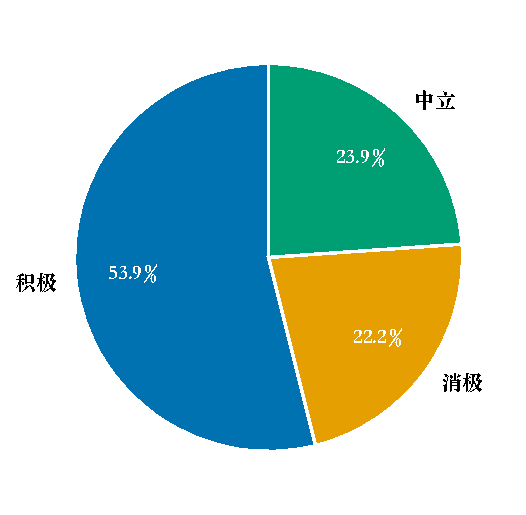
\includegraphics[width=0.55\linewidth]{charts/fig_chart6.pdf}
\par\vspace{2pt}{\small 图2-9\quad 《人民日报》官方微博环境报道情感倾向占比}
\end{figure}

（三）环境议题分布

在报道议题方面，常规议题报道共有1142篇（69.3\%），突发性议题报道共有428篇（26.0\%），周期性议题报道共有77篇（4.67\%）。虽然常规议题报道仍占据主导地位，但其在整体报道中的占比相较于《人民日报》纸质版大幅降低，其让位于突发性议题报道的数额，各类突发性报道污染议题的数量在样本采集中格外显著，以日本排污事件相关报道为典型代表。

而在细分二级议题之中，传统纸面报道与新媒体平台报道也出现了类似的分歧。在细分二级议题之中，生态区或生物多样性类（21.7\%）、环境政策法规类（14.6\%）、公众参与类（11.5\%）三项议题占据前三，合计47.8\%。相较于《人民日报》纸质版中高达25.4\%的政策法规议题占比，其他种类的议题均有所上升，其中以核与辐射污染防治类、公众参与类、环境宣传教育类、大气污染防治类上升最大，分别由原先占比0.4\%、1.8\%、1.9\%、4.4\%，上升至5.83\%、11.5\%、9.41\%和11.5\%。纵观《人民日报》微博内容，也可以显然观测到其更多在环境类议题的设置偏差，其内容风格更倾向于柔性的情感化宣传，更倾向于进行宣传教育，促进公众参与环境传播实践活动，同以往纸面报道中偏硬的长篇文字报道具有极大反差。

《人民日报》的纸面报道和新媒体端的环境传播宣传议题分布确有偏差和分歧，并没有实现完美的对接，\footnote{黄河,
  刘琳琳. (2014).
  环境议题的传播现状与优化路径------基于传统媒体和新媒体的比较分析.
  国际新闻界, 36(01),90-102,p.96.}《人民日报》在新媒体平台上的环境议题分布，更多呈现出对于媒介形式的适应性，而不是对于纸面报道传统的完全延续。

\subsubsection{二、《人民日报》官方微博环境报道的话语特性}\label{ux4e8cux4ebaux6c11ux65e5ux62a5ux5b98ux65b9ux5faeux535aux73afux5883ux62a5ux9053ux7684ux8bddux8bedux7279ux6027}

（一）轻文字而重图片与视频

随着数字技术基础的铺垫，生产门槛的降低，短视频的受众范围得以下沉，短视频传播进入细水长流的常态化发展，\footnote{彭兰.
  (2019). 短视频:视频生产力的``转基因''与再培育. 新闻界,
  1,34-43,pp.34-36.}以《人民日报》为代表的主流媒体逐渐将短视频作为一种重要的公共性传播手段。短视频碎片化叙事、场景化聚焦、情感化表达的特征同样在环境类新闻方面有所体现。相较于纸面报道使用文字作为主要表达手段，《人民日报》微博端因微博平台网络字数限制，整体使用少量叙述文本搭配短视频、图片与图表进行环境保护宣传。《人民日报》微博端在环境新闻方向多媒体运用极大程度上实现了多种叙述方式的融合，对传统报纸平面传播的方式进行了突破------相较以往以文字叙述，其将传播诉诸受众的多个感官系统，注重混合情感传播模式，以情感传播为外在驱动和影响诉求\footnote{张志安,彭璐.
  (2019).
  混合情感传播模式:主流媒体短视频内容生产研究------以人民日报抖音号为例.
  新闻与写作, 7,57-66,pp.62-65.}。就环境传播常规议题报道的具体视频而言，使用美轮美奂的自然生态实景、可视化的生态破坏恶果、简短科普视频或将自然生态实拍场景同污染恶化场景进行对比呈现，以激起受众对自然生态的感官审美与对环境破坏场景的情感厌恶，是其进行环境传播视频设置的主要方法。

（二）发布零碎而整体数量少

就发布时间而言，《人民日报》微博端关于环境新闻的发布以常态化宣传为导向，体现在报道议题上则是注重于常规议题报道------即对保护生态环境的倡议、生态保护政策的解读、生态知识的普及等内容更加充实。微博端的网络传播不受限于传统纸质报道的版面设计和印刷时限，但在环境议题上，其推送仍呈现出零碎化的发布模式。与纸媒每日固定版面的集中式专题报道相比，《人民日报》微博端往往在不同时段、不定频次地发布环境类内容，将其内容穿插于其他类型的内容之间，贴合用户碎片化浏览习惯。最终呈现出高频但零散的环境类新闻推送方式，既保持了用户对环境话题的持续关注，又避免了因过度环境宣传而产生的``信息疲劳''。

而在周期性报道中，其又呈现出爆发式的发布状态。如典型的周期性报道案例------每年4月22日世界地球日的内容发布，2024年4月22日仅一日就发布了8篇推送，集投票、视频、组图、长图等多个内容形式。2023年则是13篇。每年不均一，但相较于传统纸媒时代环境报道的设置，其在数量上有了重大的突破。

（三）单向撒播到双向互动

与纸面媒体单向撒播不同，《人民日报》微博端充分利用评论区、投票功能及话题征集等互动机制，鼓励网友参与环境话题讨论。例如，在发布``塑料减量''科普视频后，常附带``你家都怎么分类塑料垃圾？''的提问，引发大量网友分享自身经验；在气候变化等重大议题的长微博末尾，则设置``点亮绿色地球·转发送暖''活动，通过点赞获取保温杯等小奖品的形式激励转发行为。借助这种问题讨论式传播，微博端不仅扩大了报道的影响力，也在一定程度上推动了公众环保意识和实际参与度的提升，增强了环境传播在促进公民环保意识发展的作用。其常在环境新闻有关内容尾部加注\#生态文明建设\#、\#碳中和\#、\#保护地球\#等话题标签，建立相应的超级话题------这些标签和超级话题不仅帮助读者在海量信息流中快速定位环境类内容，也促进了不同用户和机构的转发、讨论与二次创作。

本研究立足于环境传播视角，将《人民日报》1949---2024年间的环境报道作为历时分析样本，通过结合内容分析与话语分析方法系统考察新中国成立75周年来主流媒体环境传播的话语特征与演变脉络。论文详细分析了《人民日报》75周年纸面报道所呈现出的环境报道文本特征和宏观话语结构，并从中提炼出其所建构与反映的中国环境传播话语变迁历程，最后结合当代媒介环境，为主流媒体在新媒体平台和传统纸媒时代的环境话语建构特征和方法做了简要对比。

在文本特征层面，通过对变量的描述性分析与交叉分析，研究发现主流媒体在75周年间环境新闻布置存在传播文本偏硬、情感偏积极、议题分布集中等特征。通过对其关涉主体和信源的分析，发现其更多秉持主流媒介惯有责任，在环境领域作为政府和群众之间的译介而存在。

在宏观话语层面，本研究识别出75周年来主流媒体环境报道所具有的``制度理性''\,``生态文明''\,``国家叙事''\,``技术赋能''\,``经济争夺''与``风险对抗''六大主要报道框架，并由此将样本进行归类解读。《人民日报》在不同历史时期对这些框架的运用各有侧重，但``制度理性''框架贯穿始终，``生态文明''框架则在近年来越发凸显，初步勾勒出主流媒体环境报道策略从早期侧重法制建设、国家叙事，到中期融入技术视角，再到新时代突出生态文明理念的演进轨迹。

基于本文前段的文本特征分析和宏观话语分析结果，本研究所进行的话语实践分析进一步揭示了中国主流媒体环境话语反映与建构出的四个关键演变阶段------从新中国成立初期将环境视为``公共卫生''的附属性议题、到改革开放后将其纳入法制轨道，逐渐走向中心舞台的``法制筑基''阶段、再到强调科学发展观，以技术创新应对环境挑战的``技术为核''阶段、最终发展至当今将生态文明建设置于核心地位，倡导全社会参与的``共治目标''阶段------对中国新中国成立以来环境话语的变迁历程做了清晰的爬梳。

本文最后基于《人民日报》微博端环境新闻报道内容及其话语实践特征，同传统纸面报道分析结果做了简要对比，发现新媒体平台继承了纸媒的核心立场和对国家政策的聚焦，但在话语表达形式、议题呈现类型上表现出新的特点，展现了主流媒体在融合媒体时代进行环境传播的改变与创新。

\section{第三章
视觉叙事与环境话语建构}\label{ux7b2cux4e09ux7ae0-ux89c6ux89c9ux53d9ux4e8bux4e0eux73afux5883ux8bddux8bedux5efaux6784}

20世纪60年代，随着环境运动在西方社会的兴起和发展，``环境''逐渐成为研究者们关注的显要问题。在传播学领域，德国社会学家尼克拉斯·卢曼（Niklas
Luhmann）于1989年最早提出``环境传播''的概念并将其定义为：``旨在改变社会传播结构与话语系统的任何一种有关环境议题表达的传播实践与方式''\footnote{Luhmann,
  N. (1989). \emph{Ecological Communication}. Trans. John Bednarz.
  Chicago, IL: University of Chicago Press, p. 28.}。这一定义表明，环境传播研究关注的核心是考察关于环境的媒介表征及其演变过程，以及在过程中所形成的符号阐释和话语建构问题。换言之，环境议题研究的首要关注点是要把握生产和建构环境话语的文化语境及其话语实践过程。当今社会，随着媒介技术的不断革新，视觉逐渐取代文字成为建构环境话语的重要表征符号，在环境传播学者安德斯·汉森
（Anders
Hansen）看来，出现在公共场域中的``环境''其实是一种视觉词汇。因为无论人们如何对环境进行言说和书写，在进行文字生产之前必然伴随着人们在视觉层面对于环境的观看和感知，由此才能激活其言说的渴望，也因此，汉森认为对环境话语形成过程中的图像表征及其叙事方式的关注有助于拓展环境传播的理论资源和研究图景。\footnote{Hansen,
  A. (2011). Communication, media and environment: Towards reconnecting
  research on the production, content and social implications of
  environmental communication. \emph{International Communication
  Gazette}, 73(1-2), 7-25.}

伴随着电视、杂志以及电影等视觉媒介形态的发展以及环境视觉作品的增加，研究者们逐渐将视觉纳入到环境传播的考察范畴中。其中，视觉媒介如何讲述``自然''故事以及如何建构环境话语是研究者们关注的主要议题。学者们通过对有关环境的电视新闻报道\footnote{Cottle,
  S.(2000). TV news, lay voices and the visualisation of environmental
  risks. In Stuart Allan, Barbara Adam, and Carter Carter. (Eds),
  \emph{Environmental risks and the media}(pp.29-44). London:Routledge.}、广告\footnote{Ferrari,
  M. P. (2013). Sporting nature (s): Wildness, the primitive, and
  naturalizing imagery in MMA and sports advertisements.
  \emph{Environmental Communication:A Journal of Nature and Culture,}
  7(2), 277-296.}等视觉文本进行考察，指出媒体机构在使用视觉符号表征环境时，呈现自然环境的图像往往以一种去政治化的、奇观的以及``受到威胁''的叙事视角出现在公共领域中。有研究者进一步指出，电视以及其他视觉媒体在可视化地球、环境议题时越来越倾向于使用一种去语境话的、抽象的视觉图像，以此构建能够被不同文化、地域的人们所普遍认可的认知符号与叙事文本，相应地也形成了一种以``全球想象''为叙事核心的环境话语。\footnote{Linder,
  S. H. (2006). Cashing-in on risk claims: On the for-profit inversion
  of signifiers for ``global Warming''. \emph{Social Semiotics}, 16(1),
  103-132.}对此，汉森等人认为，去语境话的环境图像及其视觉叙事在将环境可见的同时，也使人们失去了将环境与特定的文化、地理以及历史环境相关联的认知能力，环境由此成为消费以及资本主义逻辑发展下的产物。\footnote{Hansen,
  A. \& Machin, D. (2013). Researching Visual Environmental
  Communication. \emph{Environmental Communication}, 7(2), 151-168.}与此同时，部分研究者发现，尽管视觉能够呈现一定程度的环境面貌，但环境也存在着无法可见化以及缓慢变化的特性，这使得相较于文字表达，视觉符号在表征环境时处于更复杂的境地。对此，具有代表性的研究是学者詹妮弗·皮普斯（Jennifer
Peeples）关于越南战争中化学污染的研究。越南战争时期，美国军方曾在越南境内大量使用了一种名叫``橙剂''（Agent
Orange）的无色无味的化学药剂除草，这种化学物质对环境以及人们的生命健康产生了严重的危害和影响。皮普斯通过梳理关于``橙剂''的图像报道后发现，正是基于``橙剂''透明性，使得环境图像在美学呈现上较为单一，因此如何展开视觉叙事成为人们理解环境议题的关键。\footnote{Peeples,
  J. (2013). Imaging Toxins. \emph{Environmental Communication}, 7(2),
  191-210, pp.205-206.}这一发现表明环境图像具有不确定性和模糊性，图像再现并不等现实环境自身，其意义建构与符号认知受到视觉叙事的影响，后者又嵌套在由民族、性别、种族组成的文化结构中。此外，还有研究者关注到了图像与社会公共参与之间的关联。例如传播学者凯文·迪卢卡（Kevin
Deluca) 提出了``图像事件''（image
events）的概念，用以强调环境图像并非仅仅作为奇观或者插图而存在，相反，图像可以作为凝聚点推动人们情绪的迸发以及行动的联结。\footnote{DeLuca,
  K. M. (1999). \emph{Image Politics: The New Rhetoric of Environmental
  Activism}. New York: the Guilford Press, p.14.}面对发生在中国的图像事件以及``绿色公共话语''实践，刘涛指出环保组织分别征用了风景图片、政治漫画以及新闻摄影这三种图像符号并形成了相应的叙事策略。\footnote{刘涛.
  (2012). 图像政治：环境议题再现的公共修辞视角. 当代传播, 2, 23-26.}

综上，可以发现，尽管现有研究对环境的视觉符号表征及其话语建构进行了有益的探索，但这些研究主要聚焦于新闻图像、广告、电视等视觉文本。当下，面对不断革新的媒介技术发展环境，视觉符号表达呈现出更为多元的媒介面貌，也由此形成了更为复杂的叙事结构。基于此，本文将聚焦于融媒体时代新型主流媒体媒介表征形式，结合具体的环境传播案例，进一步考察环境相关的视觉叙事表达及其话语建构过程。

\section{第四章
环境话语建构的多模态分析：基于视觉叙事的分析模型}\label{ux7b2cux56dbux7ae0-ux73afux5883ux8bddux8bedux5efaux6784ux7684ux591aux6a21ux6001ux5206ux6790ux57faux4e8eux89c6ux89c9ux53d9ux4e8bux7684ux5206ux6790ux6a21ux578b}

正如前文所述，伴随着媒介技术的迭代与革新，环境话语建构也不再依赖于单一的表征符号，相反，融合媒介成为再现环境议题的主要形式。这一媒介形式也使得环境话语分析面临新的挑战，基于单一文字或图像符号的话语分析已经无法适用于当下的环境话语文本。由此，多模态话语分析为把握新媒介时代的环境话语提供了有益的理论视角。``多模态''（multimodality）理论发端于20世纪90年代，依照该理论的代表学者甘瑟·克雷斯（Gunther
Kress）的定义，模态（mode）指的是意义生产所采用的、基于社会文化所塑造的符号资源，诸如图像、言语、视频、姿态、音乐等都可看作是用于表征的模态。\footnote{Kress,
  G.(2010). \emph{Multimodality: A Social Semiotic Approach to
  Contemporary Communication}. London: Routledge, p.84.}基于此，多模态话语即指由两种或多种符号参与编码以及意义建构的复合话语。而针对话语文本中的符号系统或复合模态及其所构成的整体意义进行分析的方式也被称为``多模态话语分析''。

在叙事研究层面，面对数字叙事、跨媒介叙事等新兴叙事形态所呈现的动静态影像文本、非线性叙事或互动叙事等叙事文本与叙事实践，多模态话语分析成为人们理解新媒介叙事形态的叙事结构及其话语建构重要途径。在多模态理论研究者露西·佩吉（Ruth
Page）看来，多模态的分析视角也使在传统叙事中一直被忽视的媒介性、感官性以及物质性等分析纬度得以重新进入到研究者的分析视野中。\footnote{Page,
  R.(2010). Introduction. In Ruth Page(Ed.). \emph{New Perspectives on
  Narrative and Multimodality}. New York: Routledge, p.6.}当下，环境视觉产品往往经由多种媒介与模态组合配置而成，面对这一复杂形态，我们该如何理解视觉文本中的模态表征及其意义生产？又该如何理解多种模态的相互作用与环境话语建构间的关系？对此，由语言学家克莱尔·佩因特（Clare
Painter）、吉姆·马丁（Jim Martin）和伦·恩斯沃斯（Len
Unsworth）所提出的视觉叙事多模态分析模型为回应上述问题提供了有效的进入路径。

视觉叙事分析模型的提出受到语言学的影响。在语言学领域，英国语言学者迈克尔·哈利德（Michael
Halliday）提出语言具有三大元功能，即概念功能（ideational
function）、人际功能（interpersonal function）和语篇功能（textual
function）\footnote{Halliday, M. A. K.(1978). \emph{Language as social
  semiotic: The social interpretation of language and meaning}. London:
  Edward Arnold, p.183.}，这三大功能被用以理解语言的意义系统，并对人们认知视觉产生了深远影响。在此基础上，1996
年，克雷斯和西奥·凡·勒文（Theo van Leeuwen）在其著作《解读图像:
视觉设计的语法》（Reading Images：The Grammar of Visual
Design）中，将语言结构中的语法框架延伸至视觉领域，开创性地提出了视觉语法的概念，为图像系统提供了重要的阐释框架。克雷斯与凡·勒文提出在视觉层面同样存在三种图像符号的意义系统，即表征意义（representational
meaning）、互动意义（interactive meaning）以及构图意义（compositional
meaning）。不同的意义系统对应的是不同的视觉语法的分析过程，比如表征意义关注的是图像文本中的视觉元素构成及其叙事关系\footnote{Kress,
  G. \& van Leeuven, T. (2006). \emph{Reading images: The grammar of
  visual design (2nd edition)}. London: Routledge, p.59.}；互动意义关注图像提供者如何吸引观看者的注意力，以及他们之间存在怎样的关系问题\footnote{Kress,
  G. \& van Leeuven, T. (2006). \emph{Reading images: The grammar of
  visual design (2nd edition)}. London: Routledge, p.74.}；构图意义则聚焦于揭示整体层面不同视觉要素的布局结构及其意义表达\footnote{Kress,
  G. \& van Leeuven, T. (2006) . \emph{Reading images: The grammar of
  visual design (2nd edition)}. London: Routledge, p.149.}。视觉语法的分析模式也为多模态话语理论奠定了基础。在对视觉语法的深入探索过程中，研究者们逐渐意识到克雷斯与凡·勒文等人提出视觉语法框架并非适用于所有图像形式。新媒介时代，包含声音、图像、文字、动画等多种媒介符号的视觉作品的出现，也挑战着视觉语法部分框架的适用性和合理性。

对此，佩因特、马丁以及恩斯沃斯这三位语言学者展开了进一步的尝试。他们在2013年出版的著作《解读视觉叙事：儿童图画书的图像分析》（Reading
Visual Narratives: Image Analysis of Children's Picture
Books）中，发展了克雷斯与凡·勒文的语法框架，提出针对复合图像构成的视觉叙事分析模型，可以从概念意义（Ideational
meaning）、人际意义（interpersonal meaning）和语篇意义（textual
meaning）这三个视觉系统来理解视觉叙事中的符号组成与意义架构。\footnote{Painter,
  C., Martin, J., \& Unsworth, L. (2013). \emph{Reading visual
  narratives: Image analysis of children\textquotesingle s picture
  books}. Sheffield, UK: Equinox Publishing Ltd.}相较而言，佩因特等人提出的视觉叙事分析框架将人物塑造、情感表征等因素纳入到图像的分析系统中，更适用于涉及多模态表征和组合的视觉话语分析。此时，视觉叙事文本中的分析模态对象并非仅仅是文字、声音、图像等文本资源，还包含荧屏、数字屏幕、电话等发布平台；公开场所、私密空间、室内室外等物理环境以及听觉、味觉、嗅觉、视觉等感官模态。\footnote{Page,
  R.(2010). Introduction. In Ruth Page(Ed.). \emph{New Perspectives on
  Narrative and Multimodality}. New York: Routledge, p.7.}借助视觉叙事这一多模态分析模型，我们得以进一步考察新媒体时代的环境视觉话语实践。当下，伴随着新媒介技术形式，政府、环保组织等主体在建构环境议题时，在使用传统新闻图片、风景图片外，还常常采用互动游戏、数字新闻以及虚拟技术的视觉形式，这使得在环境话语的建构过程中，视觉作品呈现出更为复杂的叙事形态和叙事策略。

\section{第五章
新主流媒体环境话语建构的视觉叙事策略------以绿色发展话语建构为例}\label{ux7b2cux4e94ux7ae0-ux65b0ux4e3bux6d41ux5a92ux4f53ux73afux5883ux8bddux8bedux5efaux6784ux7684ux89c6ux89c9ux53d9ux4e8bux7b56ux7565ux4ee5ux7effux8272ux53d1ux5c55ux8bddux8bedux5efaux6784ux4e3aux4f8b}

正如前文所述，环境话语的建构嵌套在社会政治、经济、文化结构中。对于中国的环境话语实践而言，在不同历史阶段，人们对于环境的认知也呈现出不同的话语面貌。例如在国家环境治理方面，环境的治理话语经历了从环境治理仅仅作为``卫生''治理而存在，到环境保护作为一种独立政策话语被提出，再到环境治理开始强调行政管理与公众意识的捆绑，再到21世纪以来环境治理与共建``美丽中国''相关联的话语演变。\footnote{刘琳琳,黄河.
  (2022). 新中国成立以来政府环境治理话语的演变与发展. 国际新闻界,
  44(02), 58-77, pp.61-66.}环境治理决策定制的背后反映的是不同历史时期中国社会对环境问题的认知差异，以及不同认知观念对环境议题媒介话语实践的影响。有研究者指出新中国成立70年，在主流媒体环境报道中共出现了包括环境卫生、国家主权、经济争夺、制度理性、技术治理以及生存危机在内的七种话语生产框架模式。\footnote{李娜.
  (2019). 从爱国到文明：讲过70年主流媒体环境话语变迁与共意动员. 新闻界,
  12, 38-49, pp.41-44.}郭小平等人提出，环境的媒介话语建构和推动往往是由政府、主流媒体机构、NGO组织以及社会公民等多元主体共同完成，但在环境实践的不同阶段，话语建构的主导性力量也在不断发生变化。\footnote{郭小平,
  李晓. (2020).
  环境议题的``能见度''之变与电视话语建构------以央视《新闻调查》(2000---2019)为例.
  厦门大学学报(哲学社会科学版), 2, 41-51, p.48.}当下，由政府主导的``生态文明''\,``可持续发展''重新成为环境话语建构的主导性话语，为环境议题的视觉叙事提供了``政治合法性''。\footnote{郭小平,
  李晓. (2020).
  环境议题的``能见度''之变与电视话语建构------以央视《新闻调查》(2000---2019)为例.
  厦门大学学报(哲学社会科学版), 2, 41-51.}党在十八大正式将``生态文明''提升至与``经济建设、政治建设、文化建设、社会建设''同等重要的总体布局中。\footnote{胡锦涛.
  (2012). 坚定不移沿着中国特色社会主义道路前进
  为全面建成小康社会而奋斗------在中国共产党第十八次全国代表大会上的报告.
  人民网,
  \url{http://cpc.people.com.cn/n/2012/1118/c64094-19612151-7.html,}
  2022年8月6日访问.}党的十九大指出，生态文明建设需要建立``尊重自然、顺应自然、保护自然''的哲学伦理认知以及``社会主义生态文明观''的政治认知，并要践行``绿水青山就是金山银山''与``绿色发展''的实践理念。\footnote{习近平.
  (2017). 决胜全面建成小康社会
  夺取新时代中国特色社会主义伟大胜利------在中国共产党第十九次全国代表大会上的报告.
  中国政府网,
  \url{http://www.gov.cn/zhuanti/2017-10/27/content_5234876.htm?gs_ws,}
  2022年8月6日访问.}在传播学者赵月枝等人看来，相较于充斥着资本主义意识形态以及生态危机论调的西方环境话语，中国``生态文明''的国策和建设更具革新意义，这一观点打破了人-自然二元对立的既有框架，强调``人与自然和谐共生''的基础认知。\footnote{赵月枝,范松楠.
  (2020).
  环境传播理论、实践与反思------全球视角下的环境正义、公众参与和生态文明理念.
  厦门大学学报(哲学社会科学版), 2, 28-40, p.36.}可以说，生态文明建设的提出不仅作为一种与国家发展、治理相关联的顶层设计方针，更是作为一种话语形式需要被政府、公众、公益组织、资本、技术等多方主体所认知和实践。

诚如前文所探讨的，环境议题的媒介呈现往往与媒介形式有着紧密关系。如果说``卫生''治理时期，报纸承载的是环境议题再现功能，那么在新媒体时代，伴随着人们对pm2.5等环境生活的关注与争议，微博等媒体则成为环境议题的舆论场。当前，在融媒时代，人们越来越明确绿色发展不仅意味着对环境的治理，更重要的是人与环境的和谐发展。\footnote{二十大}这也对主流媒体的环境报道与呈现提出更高要求，即媒体不能止步于环境议题的呈现和舆论组织，而是促进人们通过行动深入参与、介入到环境生活中，从而理解绿色发展与社会、个人生活的关系。伴随着移动智能手机等终端媒介的发展，H5、网页游戏、VR（Virtual
Reality）、AR（Augmented
Reality）、短视频等媒介载体则为主流媒体建构绿色发展话语提供了丰富的媒介形式；与此同时，多模态的视听语言也进一步拓展了环境话语视觉叙事的表现空间。基于此，本文将聚焦绿色发展议题的典型案例，具体探讨融媒体时代环境话语的视觉叙事。

\subsection{第一节
概念意义：``交互行动-绿色认知''的叙事表征}\label{ux7b2cux4e00ux8282-ux6982ux5ff5ux610fux4e49ux4ea4ux4e92ux884cux52a8-ux7effux8272ux8ba4ux77e5ux7684ux53d9ux4e8bux8868ux5f81}

在克雷斯与凡·勒文提出的视觉语法系统中，概念意义框架关注的某种概念或话语是如何在视觉层面被呈现以及被人们所认知的。\footnote{Kress,
  G. \& van Leeuven, T. (2006). \emph{Reading images: The grammar of
  visual design (2nd edition)}. London: Routledge, pp.44-76.}克雷斯与凡·勒文强调叙事是视觉话语的表征形式之一，图像叙事即指对正在发生事件的再现，而构成图像叙事成立的关键则是矢量（vector）的出现。\footnote{Kress,
  G. \& van Leeuven, T. (2006). \emph{Reading images: The grammar of
  visual design (2nd edition)}. London: Routledge, p.55.}在图中，矢量指的是一种具有方向性的描述符号，它可以是线条、图形、身体亦或者局部肢体构成，用于表明不同视觉要素之间的指向性关系。\footnote{Kress,
  G. \& van Leeuven, T. (2006). \emph{Reading images: The grammar of
  visual design (2nd edition)}. London: Routledge, p.55.}克雷斯与凡·勒文借用语言结构关系，指出具有方向性的矢量过程可以看作是语言结构中的动词，而图像中呈现的人、物、图标等``参与者''（participants）要素则充当着名词的作用，由此便在视觉层面中形成了一种图像性的叙事结构。\footnote{Kress,
  G. \& van Leeuven, T. (2006). \emph{Reading images: The grammar of
  visual design (2nd edition)}. London: Routledge, p.75.}在此基础上，佩因特等人进一步发展了概念意义的框架系统，提出视觉叙事的过程除了涉及参与者、过程要素外，还应包含环境要素。\footnote{Painter,
  C., Martin, J., \& Unsworth, L. (2013). \emph{Reading visual
  narratives: Image analysis of children\textquotesingle s picture
  books}. Sheffield, UK: Equinox Publishing Ltd, pp.55-83.}换言之，视觉叙事需要关注图像中的人物表征特征、事件关系特征以及环境关系特征，它们构成了理解视觉叙事的关系网络。\footnote{冯德正.
  (2015). 视觉语法的新发展：基于图画书的视觉叙事分析框架. 外语教学,
  36(03), 23-27, pp.25-26.}这一关系网络也有助于我们把握主流媒体绿色发展话语的视觉叙事系统。下文将以新华网智库``思客''制作的数字新闻作品《大河奔流------黄河流域生态保护和高质量发展》（下文简称《大河奔流》）为例进一步说明。

《大河奔流》为讲述直观、具体的母亲河------黄河的生态保护与可持续发展对人类社会的影响这一重要命题，综合运用VR全景、手绘长图、数据分析、H5以及竖屏互动视频等形式。可以发现，借助于新闻的互动设计，《大河奔流》试图向人们讲述和传达的是一个``个体通过参与互动，认知到绿色发展的话语观念，并将其付诸行动''的视觉故事。聚焦《大河奔流》第五章``流动史诗''（见图5-1），借助概念意义叙事系统中的参与者、过程以及环境这三个要素，我们便可进一步《大河奔流》视觉叙事发生和运作过程。

\begin{figure}[htbp]
\centering
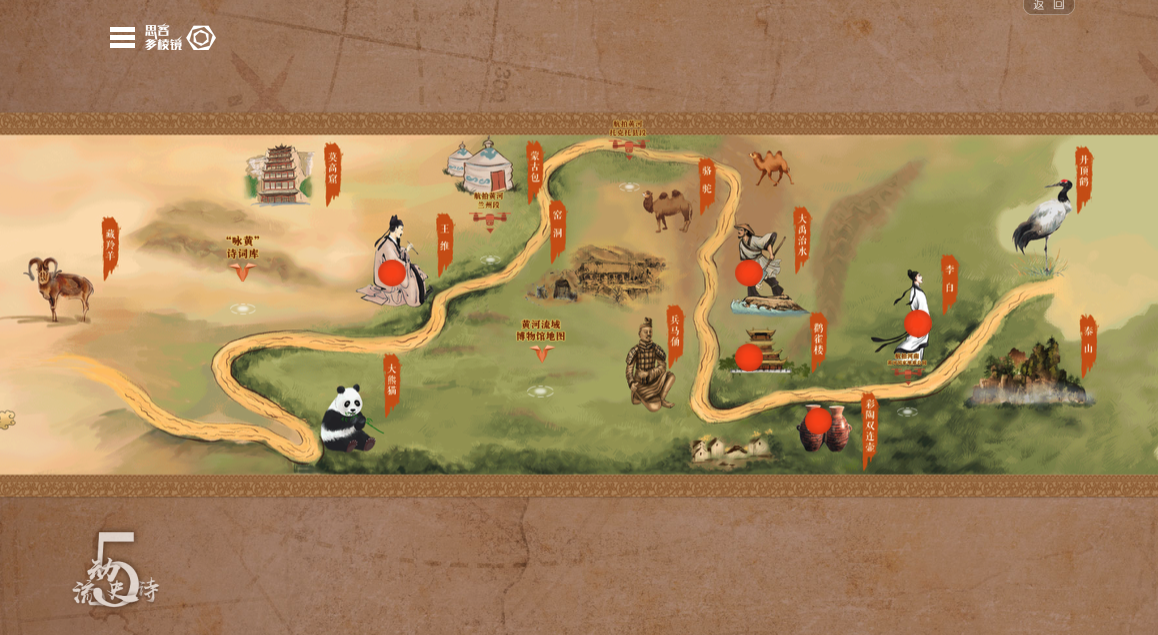
\includegraphics[width=0.8\linewidth]{media/media/image4.png}
\par\vspace{2pt}{\small 图5-1\quad 《大河奔流》第五章“流动史诗”局部截图}
\end{figure}

首先，从``流动史诗''这一章的起始界面来看，图像包含多种参与叙事的视觉元素。这些视觉元素包括在界面中心所呈现的以手绘动画形式出现沿着黄河河流的不同地域节点所出现的各个地区代表性的历史人物，动物、建筑等具体形象，每个形象上方附加一个不断闪动的红点图标提示受众可根据自己的兴趣选择相应内容，以便进一步浏览相关内容。在界面右侧和底侧所展示则是章节标题以及返回图表。

这些可见的视觉元素共同构筑了人们将``流动史诗''手绘动画界面与环境、黄河相关联的认知语境。需要注意的是，不同于传统的二维图像，交互设计后的``流动史诗''图像中还包含另一个``不可见''的参与元素，即正在浏览观看的受众。他们即是图像界面的观看者，同时也是交互叙事的组成部分。交互界面的设置特性改变了观者对于视觉叙事的理解方式，观者不再依靠观看和想象拼接叙事逻辑，而是通过作为重要的``参与者''元素进入到视觉叙事中，由此环境故事的视觉叙事才得以完整呈现。

于是，这便促使我们进一步追问``流动史诗''的视觉故事是如何经由交互行动展开的，换言之，不同的视觉元素沿着怎样的叙事逻辑而组合，从形成一个完整的叙事内容，使人们得以理解``流动史诗''的故事发展和走向。这其中，动态化的界面图像以及互动机制的设置成为视觉叙事展开的关键：首先，``流动史诗''界面图像为受众提供了黄河沿线历史文化的视觉内容。图像中代表黄河蜿蜒曲折的黄色曲线可以看作是克雷斯与凡·勒文视觉语法框架中的具有向右箭头指向的矢量符号，这使得受众在观看主界面时便可理解曲线不同节点周围出现的建筑、动物、人物形象与黄河的关系，引发观众进入到更为具体的环境故事中的兴趣。其次，``流动史诗''的互动机制引导受众在人机交互行动中理解故事发展。在交互界面所呈现的故事内容基础上，受众进而将静态观看转向为一种界面操作，即用手指点击屏幕中闪动的红色图标进入到与动物、人物、建筑相关联的黄河生态故事中。在这一互动过程中，受众通过``我''的主体介入进一步明确了``流动史诗''所建构的视觉叙事，即黄河不仅是影响数十个省市人们生活的重要水域，更是滋养中华文明蓬勃发展的摇篮。例如当受众点击``咏黄''诗词库图标时，便可看到一副绘制了从先秦到清代为黄河书写和咏诵的著名诗人的圆形树状图。最后，基于界面的交互设置将视觉叙事内容从现实的环境生态延伸至历史文化故事，从而强化受众保护黄河生态与传承黄河文化故事的绿色认知。正如受众打开``流动史诗''这一章节时，呈现的是一幅横轴徐徐展开的``画卷''，画作的动画模拟方式也使人们将黄河生态中的水域、环境发展与人们长久以来因水而生的黄河文化相关联。这明确地向人们传递了，如果没有黄河这一独特的自然生态，也没有围绕其所形成的各个地区独特文化形态，而后者更是塑造了中华民族精神品格的重要来源。

此外，《大河奔流》的视觉叙事还包含从虚拟空间到物理空间的环境``转场''。环境的变化和差异也为个体提供了不同的叙事视角和叙事体验。如果说在虚拟动画中，受众作为互动设计的既定要素参与着视觉叙事的展开，那么通过卫星遥感图等方式提供的现实图像，则使受众更为明确地感知到黄河生态的现状以及其个体之间关联。这促使个体在叙事中的主观能动性发挥着更大作用。换言之，在基于界面的互动行动外，黄河生态的保护更需要个体的参与，受众越多的参与也意味着``交互行动''的视觉叙事与``绿色行动''的现实叙事作为整体不断地与更为宏大的``绿色发展''的话语衔接，最终实现受众对这一话语的认识和理解。

\subsection{第二节
人际意义：用户视点与情感``卷入''的叙事感知}\label{ux7b2cux4e8cux8282-ux4ebaux9645ux610fux4e49ux7528ux6237ux89c6ux70b9ux4e0eux60c5ux611fux5377ux5165ux7684ux53d9ux4e8bux611fux77e5}

人际意义关注的是叙述生产者与观者间的交流方式与认识态度。佩因特等人提出可以通过聚焦（focalization）、情感（pathos）、氛围（ambience）以及视觉极差（graduation）等视觉系统来进一步展视觉叙事中的人际意义。\footnote{Painter,
  C., Martin, J., \& Unsworth, L. (2013). \emph{Reading visual
  narratives: Image analysis of children\textquotesingle s picture
  books}. Sheffield, UK: Equinox Publishing Ltd, p.18.}其中，聚焦系统关注的是观者如何与叙事人物发生互动，以及图像生产者为观者预置了怎样的观看视点。佩因特等人认为观者观看图像时存在两种进入图像叙事的观看视角，分别是接触（contact）和旁观（observe），前者表明观者是以图像人物的视角展开图像阅读，后者则是指观者独立于图像文本，以第三者的身份进行观看。\footnote{Painter,
  C., Martin, J., \& Unsworth, L. (2013). \emph{Reading visual
  narratives: Image analysis of children\textquotesingle s picture
  books}. Sheffield, UK: Equinox Publishing Ltd, p.19.}在学者冯德正看来，接触和观察类似于电影研究中的主观镜头和客观镜头，本质强调的是不同视点观看模式下的观者对于图像叙事的认知差异。\footnote{冯德正.
  (2015). 视觉语法的新发展：基于图画书的视觉叙事分析框架. 外语教学,
  36(03), 23-27, p.24.}

在澎湃新闻推出的H5数字新闻《垃圾分类王者战，邀你来挑战！》（以下简称《垃圾分类》）（见图5-2）中，较为典型地呈现了聚焦系统下视觉叙事与受众情绪感知的关系。党的十八大以来，以习近平同志为核心的党中央将生态文明建设提升至``五位一体''总体布局的战略高度，形象地提出``绿水青山就是金山银山''的绿色发展要义。其中，垃圾治理作为环境保护的重要内容，越来越受到社会关注。十九大报告明确指出``加强固体废弃物和垃圾处置''。\footnote{习近平. (2017). 决胜全面建成小康社会 夺取新时代中国特色社会主义伟大胜利------在中国共产党第十九次全国代表大会上的报告. 人民出版社. \hl{[TODO：原稿标注``改''，请核对十九大报告引文出处与页码]}}习近平总书记更是明确指出，``普遍推行垃圾分类制度，关系13亿多人生活环境改善，关系垃圾能不能减量化、资源化、无害化处理。要加快建立分类投放、分类收集、分类运输、分类处理的垃圾处理系统，形成以法治为基础、政府推动、全民参与、城乡统筹、因地制宜的垃圾分类制度，努力提高垃圾分类制度覆盖范围。''\footnote{习近平在中央财经领导小组第十四次会议上的讲话（2016年12月21日）. \hl{[TODO：原稿标注``改''，请补充正式出处、出版信息与页码]}}在此基础上，上海于2019年7月颁布《上海市生活垃圾管理条例》，正式将生活垃圾分类纳入立法强制保障条例中。而对于普通大众而言，人们对于垃圾分类的认知还处于浅层阶段，因此，由主流媒体制作的融媒产品便成为宣传垃圾分类的重要手段。对于，澎湃新闻以新闻游戏的方式设计的互动游戏《垃圾分类》即是以游戏视觉叙事的方式让受众积极感知、参与的典型作品。

\begin{figure}[htbp]
\centering

\includegraphics[width=0.45\linewidth]{media/media/image5.jpeg}
\par\vspace{2pt}{\small 图5-2\quad 澎湃H5数字新闻作品《垃圾分类王者战，邀你来挑战！》截图}
\end{figure}

从《垃圾分类》的叙事文本来看，其游戏化的媒介特性赋予了受众作为叙事主体、独一无二的``玩家视点''。不同于文学作品与传统影视作品中的``读者/观者''，游戏玩家掌握着叙事的主导权，只有在玩家主动推动游戏情节时，叙事才能有所进展，否则将会停滞。\footnote{Grodal,
  T. (2003). Stories for Eye, Ear, and Muscles: Video Games, Media, and
  Embodied Experiences. In Mark J.P. Wolf \& Bernard Perron(Eds.),
  \emph{The Video Game Theory Reader}(pp.129-156). New York: Routledge,
  p.139.}
可以说，《垃圾分类》玩家视点的叙事设置使受众得以以第一人称视角观看游戏，在主体镜头的观看结构中把握着游戏的叙事走向。此时，游戏受众不仅仅作为游戏角色而存在，更重要的，受众还是以隐含作者的视角参与着叙事创作。这一独特的聚焦结构促使受众在《垃圾分类》游戏中获得了更为``沉浸''的叙事体验。与此同时，《垃圾分类》游戏的多媒介特性和互动属性也在不断强化受众对于叙事的沉浸和投入。游戏为受众搭建了一个仿真的虚拟场景，使受众在视觉外，还可以借助听觉、触觉等多感知系统操控游戏对象。多媒介的融合作用以及多感官调用为个体打造了一个独立的感知空间，增强了受众的``临场感''和``沉浸感''，进一步加强受众的主体感知以及对于叙事角色的认知。此外，游戏``答题-闯关''模式的设置下，受众可在不断的问答中获得即时反馈，随着虚拟成就的不断积累，引发受众进一步参加和获胜的渴望。此时，个体的角色感知延伸至现实空间，强化着受众在不同空间的叙事体验。

在佩因特等人看来人际意义中的另一个值得关注的子系统则是情感。情感召唤着观者对于图像叙事的``卷入''，而决定观者卷入程度的则是图像呈现现实的详细度和真实性。当图像的``真实''程度越高，观者调动的情绪也就越强烈。依据这一分类，佩因特等人提出图像可以被为三种风格类型，即极简（minimalist）、通用（generic）和自然（naturalistic）。\footnote{Painter,
  C., Martin, J., \& Unsworth, L. (2013). \emph{Reading visual
  narratives: Image analysis of children\textquotesingle s picture
  books}. Sheffield, UK: Equinox Publishing Ltd, p.30.}其中极简风格指的是诸如简笔绘画形成的再现图像，较为抽象；通用则是指人们能够在图像中轻易识别其现实对应物的再现图像；自然则是指以``自然''\,``真实''的风格还原事物的再现图像。基于这一分类方式，可以发现，《垃圾分类》的图像再现包含着通用和自然两种风格类型，它们在不同层面作用于受众在视觉叙事过程中的情绪卷入。一方面，在游戏界面，垃圾分类的品类以一种实物图和水彩画的方式被呈现，这促使人们在观看图像时便明确了图像中的虚拟物品与真实物品之间的对应关系，个体的数字垃圾分类对应着物理世界中的现实分类，由此推动着受众参与真实垃圾分类实践的渴望；另一方面，观者进入图像叙事的情绪也在他们最终看到自己游戏奖赏时得到进一步确认和强化。根据游戏设定，受众在挑战游戏成功后，便会获得一枚``环保小卫士''电子证书，并可以``一键转发''至朋友圈进行展示。此外，用户还可获得一定额度的``正能量积分''，当积分累计至到一定程度时，便可转化为植树、送爱心等公益行动。可以发现，个体基于虚拟游戏的满足感随着游戏挑战、电子证书、公益行动等方式不断被累计和强化，《垃圾分类》的游戏互动也促使受众明确游戏所传达的个体参与与社会绿色发展话语的实践有效性，从而更为沉浸于游戏叙事中。

\subsection{第三节
语篇意义：竖屏装置与嵌入叙事的构图结构}\label{ux7b2cux4e09ux8282-ux8bedux7bc7ux610fux4e49ux7ad6ux5c4fux88c5ux7f6eux4e0eux5d4cux5165ux53d9ux4e8bux7684ux6784ux56feux7ed3ux6784}

语篇意义关注的是不同要素在图像整体层面的意义内涵与协作逻辑。克雷斯与凡·勒文认为，在构图编排中，视觉元素与文字的位置编排往往携带着不同的价值信息，部分元素因其涉及的诸如大小、色调等信息值不同，进而影响着图像构图布局。\footnote{Kress,
  G. \& van Leeuven, T. (2006). \emph{Reading images: The grammar of
  visual design (2nd edition)}. London: Routledge, pp.181-186.}在佩因特等人看来，尽管克雷斯与凡·勒文从信息价值的角度把握构图关系为人们认识图像结构提供了便利，但这一划分是否适用于全部图像类型仍具有一定争议。为了回应这一问题，佩因特等人将信息值框架完善为版面（layout）框架，并提出在视觉叙事语篇中图像和文字的关系并不能仅仅依靠左-右或者上-下的空间位置来判断，而是需要借助融合（integrated）和互补（complementary）这两种关系结构来把握。其中，前者表明语言被整合至图像中，成为图像的一部分；后者则是指语言和图像格各自占据一部分构图空间，发挥其符号学功效。\footnote{Painter,
  C., Martin, J., \& Unsworth, L. (2013). \emph{Reading visual
  narratives: Image analysis of children\textquotesingle s picture
  books}. Sheffield, UK: Equinox Publishing Ltd, pp.92-93.}

当下，基于媒介技术的发展，视觉叙事的语法规则也在不断发生变化。值得关注的是，以智能手机为代表的``竖屏''终端设备对于视觉构图产生了变革性影响。``从`宽屏'到`竖屏'的演变，表面上是一种媒介载体的形式演变，实际上揭示的则是一场普遍而深刻的`信息方式'（the
mode of
information）的变化。''\footnote{刘涛. (2021).
  新媒体竖屏叙事的``版面''语言及其语图关系. 现代出版, 5, 25-35, p.26.}竖屏的出现彻底地改变了人们的观看关系和认识方式，也影响着视觉叙事展开和观看的语法规则。对此，刘涛从修辞学的视角提出新媒体竖屏叙事形成了两种叙事方式，其中一种是并置叙事，即在竖屏图像结构中，语言和文字以一种交替出现的方式展开叙事；另一种则是嵌入关系，图像和文字互相嵌合至各自的叙事逻辑中，最终呈现出一种更为统一的叙事景观。\footnote{刘涛.
  (2021). 新媒体竖屏叙事的``版面''语言及其语图关系. 现代出版, 5, 25-35,
  pp.29-30.}相较而言，刘涛提出的并置与嵌入的叙事模式与佩因特等人提出的融合和互补的版面框架具有一定的相似性，都关注了语图关系间的结构差异对叙事法则的影响，但不同的是，刘涛更强调竖屏这一新的视觉再现装置在视觉叙事过程中的决定性作用。从这一视角来看，H5等数据新闻是出现在手机装置中的独特视觉产物，其图像叙事不可避免地受到受到竖屏这一媒介物的影响。

新京报于2016年制作的H5数据新闻《一张图看懂雾霾如何由南向北攻陷北京城》（下文简称《一张图》）便是利用竖屏结构展开叙事的典型。如图所示，文字与图像形成了一种嵌入关系的叙述方式。尽管从图像的界面构图来看，视觉元素占据的空间比例较大，但此时，文字并非只是作为图像的``解说''或``补充''而存在，相反，文字为观者提供了不同的叙事内容，二者共同作用于雾霾随着地理不断发展变化的视觉叙事。基于图像与文字的嵌入关系，刘涛更进一步指出，竖屏中的信息呈现往往表现为对于其他媒介内容的征用和吸用，是一种``再媒介化''（remediation）过程，因此，依照媒介的形态、语法以及意象这三个纬度，竖屏中图像和语言的整合关系也表现为三种形式，即媒介形态的``信息长图''，媒介语法的``一镜到底''以及媒介意象的``时间轴图''。\footnote{刘涛.
  (2021). 新媒体竖屏叙事的``版面''语言及其语图关系. 现代出版, 5, 25-35,
  pp.32-34.}

《一张图》呈现环境叙事的媒介特性也使得其叙事结构并不局限于单一的图式关系，而是呈现出复合、杂糅的构图面貌。纵观《一张图》叙事文本中图像与文字的作用方式，显然，多种语图整合关系共同作用于环境故事的构图编排与叙事布局。首先，``信息长图''构图中的垂直空间滚动叙事（scrollytelling）。在《一张图》的新闻界面中，最左侧的时间线伴随着人们的竖屏滑动习惯不断增加，而在右侧的钟表图标、地图、实景图等文字和图像信息被整合至一个垂直的长画幅结构中，当受众进入游戏界面，只需借助手指滑动屏幕，便可获知关于雾霾由南向北气候变化的完整叙事信息。其次，``一镜到底''构图中的空间叙事。``一镜到底''是对电影``长镜头''语言的征用，强调在``一个镜头空间内模拟、缝合或呈现完整的叙事脉络''\footnote{刘涛,
  刘倩欣. (2020). ``一镜到底''：融合新闻的叙事结构创新. 新闻与写作, 2,
  74-80, p.74.}。在《一张图》中，``一镜到底''的叙事主要体现在时间序列下多场景的空间叙事对比。一方面，数据新闻以全国雾霾数据为坐标告知人们当日雾霾发展的基本情况；另一方面，在每个时间段，以央视电视台为对照场景，实时观测并反馈环境变化实物图。通过全国与央视电视台的对照和交互叙事，受众在竖屏浏览的过程中可以直观地感受到雾霾侵入北京的过程和变化。由此，由此，全面的图文信息、流畅的视觉观看体验以及具有社交属性的转换空间协同作用，使受众在观看长图、社交互动的过程中逐步完善叙事线索，在语图关系铺设的多种构图逻辑中不断加深对于环境污染与绿色发展治理的叙事认知，以此增强叙事效果以及受众参与的行动意愿。

综上，通过对视觉叙事模型的应用与分析，我们得以从概念意义、人际意义以及语篇意义这三个视觉叙事系统出发，把握视觉叙事的基本认知框架与意义构筑机制，进而为更深入地理解当下环境话语的视觉建构提供了有益的方向。可以发现，在新媒体技术语境下，视觉的叙事逻辑受到竖屏装置、人机交互等技术特性的影响，开始将受众、互动技术纳入到叙事过程中，由此使得视觉叙事在文本、表征、构图等方面呈现出不同的视觉形态，也由此影响着人们对于环境话语的感知及其实践。
